\documentclass[preprint,9pt,nocopyrightspace]{sigplanconf}

\usepackage{amssymb,amsmath,amsthm}
\usepackage{latexsym}
\usepackage{graphicx}
\usepackage[usenames,dvipsnames]{color}
\usepackage{listings}
\usepackage{float}
\usepackage{multirow}
\usepackage[scaled]{helvet}
\usepackage[noend]{algorithmic}
\usepackage{mathrsfs}
\usepackage{mathpartir}
\usepackage{dsfont}
\usepackage{stmaryrd}
\usepackage{url}
\usepackage{textcomp} 
\usepackage[colorlinks=true,allcolors=blue,breaklinks,draft=false]{hyperref}
\usepackage{titlesec}
\usepackage{parskip}
\usepackage{alltt}
\usepackage{bbm}
\usepackage{alltt}
\usepackage{verbdef}
\usepackage{xspace}
\usepackage{verbatim}
\usepackage{enumitem}
\usepackage{lipsum}
\usepackage{wrapfig}
%\usepackage[strut=on,labelfont=bf]{caption}
\usepackage[usenames,dvipsnames]{xcolor}
\hypersetup{linkcolor=black,citecolor=black,urlcolor=RubineRed}

\newcounter{tags}


% \usepackage{natbib}
% \bibpunct();A{},
% \let\cite=\citep

% For turned column headers 
\usepackage{adjustbox} 
\usepackage{array}
\usepackage{booktabs}
\usepackage{multirow}
\usepackage{pifont}
 
%%%%%%%%%%%%%%%%%%%%%%%%%%%%%%%%%%%%%%%%%%%%%%%%%%%%%%%%%%%%%%%%%%%%%%
% Compiling two paper versions
%%%%%%%%%%%%%%%%%%%%%%%%%%%%%%%%%%%%%%%%%%%%%%%%%%%%%%%%%%%%%%%%%%%%%%

\newcommand{\ifext}[2]{\ifdefined\extflag{#1}\else{#2}\fi}
\newcommand{\ifcomm}[1]{\ifdefined\extcomm{#1}\else{}\fi}

\newcommand{\mute}[1]{\ifdefined\draftflag{#1} \else{} \fi}
%\newcommand{\mute}[1]{}

\usepackage{skull}

\newcounter{ToDos}
\newcounter{WarnCounts}
\newcommand{\decorateWC}{
  \stepcounter{WarnCounts}
  \marginpar{\textcolor{red}{$\skull\ \theWarnCounts$}}}

\newcommand{\decorateTD}{
  \stepcounter{ToDos}
  \marginpar{\textcolor{red}{$\textbf{TO DO}_{\#\ \theToDos}$}}}


% Skeleton for remark comments
% 1: Name, 2: Color, 3:Comment
\newcommand{\signedComment}[3]
           {\mute{\textcolor{#2}{(#1: {#3})}\decorateWC}}

% remarks
\newcommand{\todo}[1]{\mute{\textcolor{red}{(TO DO:{#1})}\decorateTD}}

\newcommand{\is}[1]{\signedComment{Ilya}{blue}{#1}}
\newcommand{\an}[1]{\signedComment{Aleks}{red}{#1}}
\newcommand{\ab}[1]{\signedComment{AB}{red}{#1}}
\newcommand{\gad}[1]{\signedComment{GAD}{red}{#1}}

\newcommand{\highlight}[1]
           {\ifdefined\draftflag{{\textcolor{red}{#1}}} \else{#1} \fi}

\newenvironment{draft}
           {\ifdefined\draftflag \par\color{red} \else \comment \fi}
           {\ifdefined\draftflag \decorateWC\par \else \endcomment \fi}
           
% useful macros
\newcommand{\asgn}{\leftarrow}
\newcommand{\code}[1]{\lstinline[basicstyle=\small\ttfamily]{#1}}
\newcommand{\ccode}[1]{\lstinline[basicstyle=\footnotesize\ttfamily]{#1}}
\newcommand{\cccode}[1]{\lstinline[basicstyle=\scriptsize\ttfamily]{#1}} 
\newcommand{\Code}[1]{\code{#1}}
\newcommand{\etc}{\emph{etc}}
\newcommand{\ie}{\emph{i.e.}\xspace}
\newcommand{\id}{\emph{Id.}\xspace}
\newcommand{\eg}{\emph{e.g.}\xspace}
\newcommand{\vs}{\emph{vs.}\xspace}
\newcommand{\etal}{\emph{et~al.}\xspace}
\newcommand{\adhoc}{\emph{ad~hoc}\xspace}
\newcommand{\viz}{\emph{viz.}\xspace}
\newcommand{\dom}[1]{\mathsf{dom}(#1)}
\newcommand{\aka}{\textit{a.k.a.}\xspace}
\newcommand{\cf}{\textit{cf.}\xspace}
\newcommand{\wrt}{{wrt.}\xspace}
\newcommand{\Iff}{{iff}\xspace}
\newcommand{\loef}{L\"{o}f}
\newcommand{\sep}{\textasteriskcentered}
\newcommand{\res}{\mathsf{res}}
\newcommand{\bal}{\mathit{bal}} 
\newcommand{\ret}{\mathsf{ret}} 
\newcommand{\fix}{\mathsf{fix}} 
\newcommand{\Unit}{\mathsf{Unit}}  
\newcommand{\ic}{\mathcal{I}}
\newcommand{\Ic}[2]{\ic~{#1}~{#2}}
\newcommand{\hide}{\mathsf{hide}}  
\newcommand{\last}{\mathsf{last}}  

%specs
\newcommand{\specK}[1]{\ensuremath{\textcolor{blue}{#1}}}
\newcommand{\comm}[1]{\ensuremath{\textcolor{gray}{\esc{/\!/}~{#1}}}}
\newcommand{\spec}[1]{\specK{\left\{{#1}\right\}}}
\newcommand{\specQ}[4]{[#1 , #2 , #3] \, #4}%\specQ{mL}{gL}{gE}{p}
\newcommand{\drspec}[1]{\specK{\langle{#1}\rangle}}
\newcommand{\sspec}[1]{\specK{\{{#1}\}}}
\newcommand*{\backin}{\rotatebox[origin=c]{-180}{$\in$}}%

%actions
\newcommand{\act}[1]{\textsf{\small{#1}}}
\newcommand{\aux}[1]{\textit{#1}}
\newcommand{\Aux}[1]{\(\mathit{\small{#1}}\)}
\newcommand{\Num}[1]{{\text{{\scriptsize{#1}}}}}
\newcommand{\esc}[1]{\text{\texttt{\small{#1}}}}
\newcommand{\kw}[1]{\text{\textbf{#1}}}
\newcommand{\tp}[1]{\text{\textsf{#1}}}
\newcommand{\Asgn}{\leftarrow} 

%PCMs
\newcommand{\dotcup}{\ensuremath{\mathaccent\cdot\cup}}
\newcommand{\pcmS}{\mathbb{U}}
\newcommand{\pcmF}{\bullet}
\newcommand{\join}{\pcmF}
\newcommand{\jjoin}[1]{\ensuremath{\bigodot}_{#1=1}^n} 
\newcommand{\pcmU}{\mathbbm{1}}

% Pretty table
\newcommand{\cmark}{\ding{52}}%
\newcommand{\xmark}{\ding{55}}%
\newcommand*\rot{\rotatebox{32}} 
\newcommand{\yep}{\ding{51}}
\newcommand{\yepl}{$\text{\ding{51}}_{\!\!L}$}  
\newcommand{\yepa}{$\text{\ding{51}}_{\!\!L}$}  
\newcommand{\intab}[1]{({\sffamily{\small{#1}}})}

% Concurroids
\newcommand{\acon}{\mathcal{A}}
\newcommand{\econ}{\mathcal{E}}
\newcommand{\ucon}{\mathcal{U}}
\newcommand{\rcon}{\mathcal{R}}
\newcommand{\ccon}{\mathcal{C}}
\newcommand{\vcon}{\mathcal{V}}
\newcommand{\wcon}{\mathcal{W}}
\newcommand{\privcon}{\mathcal{P}}
\newcommand{\pscon}{\mathcal{S}}
\newcommand{\tbcon}{\mathcal{T}}
\newcommand{\fccon}{\mathcal{F}}
\newcommand{\lcon}{\mathcal{L}}
\newcommand{\alloccon}{\mathcal{A}}
\newcommand{\jayanticon}{\mathcal{J}}

%Getters
\newcommand{\lcl}{{\mathsf{s}}}%L
\newcommand{\env}{{\mathsf{o}}}%E
\newcommand{\joint}{{\mathsf{j}}}%E

\newcommand{\selfsub}{\mathsf{s}}
\newcommand{\othersub}{\mathsf{o}}
\newcommand{\jointsub}{\mathsf{j}}

\newcommand{\hist}{\chi} 
\newcommand{\histS}{\hist_{\, \selfsub}}
\newcommand{\histO}{\hist_{\, \othersub}}
\newcommand{\histJ}{\hist_{\, \jointsub}}
\newcommand{\hempty}{\emptyset}
\def\envsteps{\rightarrow^{*}_{\epsilon}}

\newcommand{\heap}{h} 
\newcommand{\heapS}{\heap_{\, \selfsub}}
\newcommand{\heapSP}{\heap_{\, \selfsub}'}

% Jayanti's Snapshot getters

\def\ordlist{\sigma}
\newcommand{\E}{\tau}
\newcommand{\C}{\kappa}


% Jayanti's Snapshot Orders
\newcommand{\tleq}{\mathrel{\leq_\ordlist}}
\newcommand{\tle}{\mathrel{<_\ordlist}}

\newcommand{\stableorder}{\Omega}
\newcommand{\prefix}[1]{-\,{\tleq}\,#1}

% Primed getters

\def\ordlistP{\sigma'}
\newcommand{\stableorderP}{\stableorder'}
\newcommand{\prefixP}[1]{(\mathrel{\tleqP}#1)}
\newcommand{\tleP}{\mathrel{<_\ordlistP}}
\newcommand{\tleqP}{\mathrel{\leq_\ordlistP}}
\newcommand{\EP}{\tau'}
\newcommand{\CP}{\kappa'}
\newcommand{\histP}{\chi'} 
\newcommand{\histSP}{\hist_{\, \selfsub}'}
\newcommand{\histOP}{\hist_{\, \othersub}'}
\newcommand{\histJP}{\hist_{\, \jointsub}'}

\newcommand{\wxP}{W_\x'}
\newcommand{\wyP}{W_\y'}
\newcommand{\wppP}{W_p'}

\newcommand{\jge}{\mathrel{>_\ordlist}}

\def\lgVy{\ensuremath{\mathsf{lastGY}}}


%% Writer and scanner states.

\newcommand{\wInit}{\mathsf{W_{Off}}}
\newcommand{\wWrite}{\mathsf{New}}
\newcommand{\wDirty}{\mathsf{Fwd}}
\newcommand{\wClean}{\mathsf{Done}}

\newcommand{\sOn}{\mathsf{S_{On}}}
\newcommand{\sOff}{\mathsf{S_{Off}}}

%mapsto stuff
\makeatletter
\newcommand{\oset}[3][0ex]{%
  \mathrel{\mathop{#3}\limits^{
    \vbox to#1{\kern-3\ex@
    \hbox{$\scriptstyle#2$}\vss}}}}
\makeatother

\makeatletter
\newcommand{\ojset}[3][0ex]{%
  \mathrel{\mathop{#3}\limits^{
    \vbox to#1{\kern-5\ex@
    \hbox{$\scriptstyle#2$}\vss}}}}
\makeatother

\newcommand{\jpts}{\mathrel{\ojset{j}{\mapsto}}}
\newcommand{\spts}{\mathrel{\oset{s}{\mapsto}}}
\newcommand{\opts}{\mathrel{\oset{o}{\mapsto}}}
\newcommand{\qcl}{\mathsf{cn}}

\newcommand{\hunion}{\mathbin{\dotcup}} 
\newcommand{\Hunion}[1]{\mathbin{\Dotcup{#1}}}

%% operators

\newcommand{\eqdef}{\mathrel{\:\widehat{=}\:}}
\newcommand{\hpts}{\mapsto}
\newcommand{\ldot}{\mathord{.}\,}

%% \newcommand{\aand}{,}
%% \newcommand{\oor}{\vee}
%% \newcommand{\nnot}{\neg}
%% \newcommand{\eqq}{\mathrel{\mbox{\tt==}}}
%% \newcommand{\neqq}{\mathrel{\mbox{\tt!=}}}
%% \newcommand{\andb}{\mathrel{\small\mbox{\&\&}}}
%% \newcommand{\orb}{\mathrel{\mbox{\tt{|\!|}}}}
%% \newcommand{\evar}[1]{?#1}
%% \newcommand{\zig}{\triangleleft}
%% \newcommand{\zag}{\triangleright}
%% \newcommand{\set}[1]{\left\{#1\right\}}
%% \newcommand{\tauflip}{\mathsf{flip\_trans}}
%% \newcommand{\tauadd}{\mathsf{add2\_trans}}
%% \newcommand{\tfr}[2]{{\text{fresh}^{#2}_{#1}}}

%% % more invariants
%% \newcommand{\tapprox}{\mathsf{ResInterf}}
%% \newcommand{\happrox}{\mathsf{ResPast}}
%% %\newcommand{\sapprox}{\mathsf{ResState}}
%% \newcommand{\bapprox}{\mathsf{ValuesMono}}
%% \newcommand{\strapprox}{\mathsf{IncResult}}
%% \newcommand{\Thisz}{\mathsf{this}}
%% \newcommand{\This}[1]{\Thisz~{#1}}

%% \newcommand{\hvalid}{\mathsf{Valid}}
%% \newcommand{\eqqc}{e_{\mathit{qqc}}}
%% \newcommand{\eqc}{e_{\mathit{qc}}}

%% \newcommand{\pending}{{m_\joint}} 
%% \newcommand{\offers}{h}
%% \newcommand{\twin}[1]{\bar{#1}}
%% \newcommand{\mygathjyer}[1]{|\!|{#1}|\!|}

%% \definecolor{shadecolor}{gray}{1.00}
%% \definecolor{ddarkgray}{gray}{0.75}
%% \definecolor{darkgray}{gray}{0.30}
%% \definecolor{light-gray}{gray}{0.87}
%% \newcommand{\whitebox}[1]{\colorbox{white}{#1}}
%% \newcommand{\graybox}[1]{\colorbox{light-gray}{#1}}
%% \newcommand{\darkgraybox}[1]{\colorbox{ddarkgray}{#1}}
%% \newcommand{\gbm}[1]{\graybox{${#1}$}}



%%% Snapshots paper related
%%%

\def\FF{\mathsf{False}}
\def\TT{\mathsf{True}}


%%% Specs
\newcommand{\tsPre}[1]{\ensuremath{{\textcolor{blue}{#1}}}}
\newcommand{\tsPos}[1]{\ensuremath{\textcolor{blue}{#1}}}
\newcommand{\logvar}[1]{\ensuremath{\textcolor{blue}{[#1].}}}

\newcommand{\var}[1]{\mathit{#1}} 
\newcommand{\num}[1]{{\text{{\scriptsize{#1}}}}}


\newcommand{\hfilter}{\mathrel{\downarrow}}

%% \newcommand{\cevX}[2]{\cev{#1}_{#2}}

%% \makeatletter
%% \DeclareRobustCommand{\cev}[1]{%
%%   \mathpalette\do@cev{#1}%
%% }

%% \newcommand{\do@cev}[2]{%
%%   \fix@cev{#1}{+}%
%%   \reflectbox{$\m@th#1\vec{\reflectbox{$\fix@cev{#1}{-}\m@th#1#2\fix@cev{#1}{+}$}}$}%
%%   \fix@cev{#1}{-}%
%% }
%% \newcommand{\fix@cev}[2]{%
%%   \ifx#1\displaystyle
%%     \mkern#23mu
%%   \else
%%     \ifx#1\textstyle
%%       \mkern#23mu
%%     \else
%%       \ifx#1\scriptstyle
%%         \mkern#22mu
%%       \else
%%         \mkern#22mu
%%       \fi
%%     \fi
%%   \fi
%% }


\def\GYR{{\mathbf{{g^{+}}{y^{?}}{r^{*}}}}}
\def\RZ{{\mathbf{{{(g | y)^{+}}}{r^{*}}}}}

%% \def\GYR{{\mathbf{{\color{OliveGreen}{G^{+}}}\bullet%
%%                    \color{YellowOrange}{Y^{?}}}\bullet%
%%                    \color{WildStrawberry}{R^{*}}}}



% code

\def\lat{\langle}
\def\rat{\rangle}
\def\tbnd{\Asgn}
\newcommand{\actwrite}[2]{{#1}\,{:=}\,{#2}}

%\def\altsubseteq{\mathbin{\subseteq}}


% Keep footnotes on one page
\interfootnotelinepenalty=10000 

\setlist[itemize]{leftmargin=*}
\setlength{\parindent}{0.15in}
\setlength{\topsep}{0cm}
\setlength{\parskip}{0pt}

\titlespacing*{\section}{0pt}{*1.5}{*1.5} 
\titlespacing*{\subsection}{0pt}{*0.8}{*0.5}
\titlespacing*{\subsubsection}{0pt}{*0.8}{*0.5}
\titlespacing*{\paragraph}{0pt}{*0.5}{*1.2}

% SSReflect listings 
% colors
\definecolor{shadecolor}{gray}{1.00}
\definecolor{darkgray}{gray}{0.30}
\definecolor{violet}{rgb}{0.56, 0.0, 1.0}
\definecolor{forestgreen}{rgb}{0.13, 0.55, 0.13}

% Col language definition
\lstdefinelanguage{Coq} {
mathescape=true,						
texcl=false,
morekeywords=[1]{
  Add,
  All,
  Arguments,
  Axiom,
  Bind,
  Canonical,
  Check,
  Close,
  CoFixpoint,
  CoInductive,
  Coercion,
  Contextual,
  Corollary,
  Defined,
  Definition,
  Delimit,
  End,
  Example,
  Export,
  Fact,
  Fixpoint,
  Goal,
  Graph,
  Hint,
  Hypotheses,
  Hypothesis,
  Implicit,
  Implicits,
  Import,
  Inductive,
  Lemma,
  Let,
  Local,
  Locate,
  Ltac,
  Maximal
  Module,
  Morphism,
  Next,
  Notation,
  Obligation,
  Open,
  Parameter,
  Parameters,
  Prenex,
  Print,
  Printing,
  Program,
  Projections,
  Proof,
  Proposition,
  Qed,
  Record,
  Relation,
  Remark,
  Require,
  Reserved,
  Resolve,
  Rewrite,
  Save,
  Scope,
  Search,
  Section,
  Show,
  Strict,
  Structure,
  Tactic,
  Theorem,
  Unset,
  Variable,
  Variables,
  View,
  inside,
  outside
},
morekeywords=[2]{
  as,
  cofix,
  else,
  end,
  exists,
  exists2,
  fix,
  for,
  forall,
  fun,
  if,
  in,
  is,
  let,
  match,
  nosimpl,
  of,
  return,
  struct,
  then,
  vfun,
  with
},
morekeywords=[3]{Type, Prop, Set, True, False},
morekeywords=[4]{
  apply,
  assert,
  auto,
  bool_congr,
  case,
  change,
  clear,
  compute,
  congr,
  cut,
  cutrewrite,
  destruct,
  elim,
  field,
  fold,
  generalize,
  have,
  heval, 
  hnf,
  induction,
  injection,
  intro,
  intros,
  intuition,
  inversion,
  left,
  loss,
  move,
  nat_congr,
  nat_norm,
  pattern,
  pose,
  refine,
  rename,
  replace,
  revert,
  rewrite,
  right,
  ring,
  set,
  simpl,
  split,
  suff,
  suffices,
  symmetry,
  transitivity,
  trivial,
  unfold,
  using,
  without,
  wlog,
  autorewrite
},        
morekeywords=[5]{
  assumption,
  by,
  contradiction,
  done,
  exact,
  lia,
  gappa,
  omega,
  reflexivity,
  romega,
  solve,
  tauto,
  discriminate,
  unsat
},
morecomment=[s]{(*}{*)},
morekeywords=[6]{do, last, first, try, idtac, repeat},
showstringspaces=false,
morestring=[b]",
% Size of tabulations
tabsize=3,							
% Enables ASCII chars 128 to 255
extendedchars=true,  		 		
% Case sensitivity
sensitive=true, 
% Automatic breaking of long lines
breaklines=false,
% Default style fors listings
basicstyle=\small\ttfamily,
% Position of captions is bottom
captionpos=b,							
% Full flexible columns 
columns=[l]fullflexible,
% Style for (listings') identifiers
identifierstyle={\color{black}},
% Style for declaration keywords
keywordstyle=[1]{\color{violet}},
% Style for gallina keywords
keywordstyle=[2]{\color{forestgreen}},
% Style for sorts keywords
keywordstyle=[3]{\color{forestgreen}},
% Style for tactics keywords
keywordstyle=[4]{\color{blue}},
% Style for terminators keywords
keywordstyle=[5]{\color{red}},
%Style for iterators
keywordstyle=[6]{\color{violet}},
% Style for strings
stringstyle=,
% Style for comments
commentstyle=\it\ttfamily\color{Bittersweet},
% Style for lines numbering
numberstyle=\tiny,
}

\lstdefinestyle{Coq}{language=Coq}
\lstset{style=Coq}

% Hyphenation
\hyphenation{Veri-Fast}

% Bibtgex tweaks
\setcitestyle{square}
\defcitealias{Coq-manual}{Coq proof assistant}

\begin{document}

%\special{papersize=8.5in,11in}


\authorinfo{Ilya Sergey \and
  Aleksandar Nanevski \and 
  Anindya Banerjee \and 
  Germ\'{a}n Andr\'{e}s Delbianco}
{IMDEA Software Institute, Madrid, Spain}
{
\{ilya.sergey, aleks.nanevski, anindya.banerjee,
  german.delbianco\}@imdea.org 
}

% \vspace{-20pt}}



% \authorinfo{}{}{}

% \conferenceinfo{PLDI~'15} {June 13--17, 2015, Portland, OR, USA}
% \CopyrightYear{2015}
% \copyrightdata{TODO}
% \doi{TODO}


%\title{The Power of Subjectivity}

\title{
  Hoare-style Specifications as Correctness Conditions\\
  for Non-linearizable Concurrent Objects
% 
%\vspace{-42pt}
}
 

\maketitle

\begin{abstract}

%
% 1. The setting
%

  Designing scalable concurrent objects, which can be efficiently used
  on multicore processors, often requires one to abandon standard
  specification techniques, such as \emph{linearizability}, in favor
  of more relaxed consistency requirements.
  %
  However, the variety of alternative correctness conditions makes it
  difficult to choose which one to employ in a particular case, and to
  compose them when using objects whose behaviors are specified via
  different criteria. The lack of syntactic verification methods for
  most of these criteria poses challenges in their systematic adoption
  and application.

  % 
  % To specify different useful classes of non-linearizable concurrent
  % objects, a number of alternative correctness criteria have been
  % proposed recently: \emph{Quiescent} and \emph{Quantitative
  % Quiescent Consistency}, \emph{Concurrency-Aware Linearizability},
  % and \emph{Quasi-Linearizability}, to name just a~few.
%
%
% 2. The problem(s): too many of correctness criteria
%
  % However, it is not trivial to design new concurrent correctness
  % conditions, which are compositional and general enough to
  % accommodate highly parallel concurrent objects.
  % 
  % It is even less trivial to supply these conditions with
  % compositional proof methods, making them amenable for structured
  % formal program verification.
  %
  % Finally, the diversity of existing specification approaches makes it
  % tricky to reason uniformly about client code that employs various
  % concurrent objects, whose semantics is defined via different
  % correctness criteria.

  % Furthermore, the clients of a concurrent data structure, when
  % committing to one or another correctness criterion, need to adopt
  % specific reasoning principles necessary to characterize the
  % structure's behavior. Therefore, client-side reasoning about
  % programs that incorporate several structures, specified via
  % \emph{different} criteria, might be tricky.
%
% 3. Our solution
%  

  In this paper, we argue for using Hoare-style program logics as an
  alternative and uniform approach for specification and compositional
  formal verification of safety properties for concurrent objects and
  their client programs.
  %
  Through a series of case studies, we demonstrate how an existing
  program logic for concurrency can be employed off-the-shelf to
  capture important state and history invariants, allowing one to
  \emph{explicitly quantify over interference} of environment threads
  and provide intuitive and expressive Hoare-style specifications for
  several \emph{non-linearizable} concurrent objects that were
  previously specified only via dedicated correctness criteria.
  %
  We illustrate the adequacy of our specifications by verifying a
  number of concurrent client scenarios, that make use of the
  previously specified concurrent objects, capturing the essence of
  such correctness conditions as \emph{concurrency-aware
    linearizability}, \emph{quiescent}, and \emph{quantitative
    quiescent consistency}.
  %
  % The compositionality of our approach follows from the
  % compositionality of the logical specifications, that abstract away
  % the implementation details and enable program substitution.
  % 
  % Using an existing logic off-the-shelf provides us with a general
  % structural verification method.
  %
  All examples described in this paper are verified mechanically
  in~Coq.

% Points to emphasize:

% \begin{itemize}

% \item Algorithms of multicore era: better scalability requires
%   rethinkin correctness

% \item Multiple ways to define correctness in some relaxed flavours, by
%   relating it to the sequential executions - name a few correctness
%   conditions

% \item These conditions are difficult to design and they are not even
%   supplied with the corresponding proof methods, which are easy
%   amenable for mechanization

% \item Furthermore, clients need to adapt their reasoning principles to
%   each of this criteria, and reasoning about programs that incorporate
%   structures with several criteria might be tricky

% \item We suggest program logic as a uniform framework for specifying
%   safety  aspects of concurrent objects 

% \item We illustrate the generality of the approach by providing
%   intuitive specifications to two concurrent objects, each of which
%   required a dedicated correctness condition to be specified

% \item Out of provided specifications, we verify a series of concurrent
%   client programs, which make use of the above described concurrent
%   objects

% \item All examples are verified mechanically in Coq

% \end{itemize}

  % \todo{Rephrase the abstract as follows: (1) keep the first paragraph
  %   (2) Outline the situation with the variety of alternative criteria
  %   and implications of this fact; (3) say, which alternative (Hoare
  %   logic) we consider and what benefits it brings; (4) mention the
  %   key observation that we need quantify over interference in order
  %   to provide concurrent specs for all these interesting concurrent
  %   objects. }

\end{abstract}

%\section{Introduction}
\label{sec:intro}

It has been long recognized that efficient parallelization is of
crucial importance for high-performant software. Unfortunately,
proving correctness of concurrent programs, in which several
computations can be executed in parallel, is difficult due to the
large number of possible interactions between concurrent
processes/threads on shared data structures.


% \ab{Can we also make the point that: fine-grained concurrent
%   algorithms are heavily used in concurrent data structure libraries
%   (cite?) and calls to such library functions in client code is
%   ubqiquitous (cite?). Therefore it is essential that the libraries be
%   proved correct. ``Verify once, use often''.}

% \is{I put this point into the abstract and added later in the intro to
%   the ``compositional" bullet of the framework description.}

One way to deal with the complexity of verifying concurrent code is to
employ the mechanisms of so-called \emph{coarse-grained}
synchronization, \ie, locks. By making use of locks in the code, the
programmer ensures mutually-exclusive thread access to critical
resources, therefore, reducing the proof of correctness of concurrent
code to the proof of correctness of \emph{sequential} code. While
sound, this approach to concurrency prevents one from taking full
advantage of parallel computations. An alternative is to implement
shared data structures in a \emph{fine-grained} (\ie, lock-free)
manner, so the threads manipulating such structures would be reaching
a consensus via the active use of non-blocking read-modify-write
operations (\eg, compare-and-swap) instead of locks.

Despite the clear practical advantages of the fine-grained approach to
the implementation of concurrent data structures, it requires
significant expertise to devise such structures and establish
correctness of their behavior.
%
%  with respect to standard criteria, such as
% \emph{linearizability}~\cite{Herlihy-Wing:TOPLAS90}.
% %
% Moreover, in the presence of advanced programming features, such
% as higher-order functions, pointer aliasing, and internal parallelism,
% linearizability by itself might not be sufficient as a criteria to
% ensure the full functional correctness of a concurrent program, and
% its generalizations to match these programming features are a topic of
% ongoing active
% research~\cite{Cerone-al:ICALP14,Gotsman-Yang:CONCUR12}.

In this paper, we focus on \emph{program logics} as a generic approach
to specify a program and formally prove its correctness \wrt the given
specification.
%
In such logics, program specifications (or specs) are represented by
Hoare triples $\spec{P}~c~\spec{Q}$, where $c$ is a program being
described, $P$ is a precondition that constrains a state in which the
program is safe to run, and $Q$ is a postcondition, describing a state
upon the program's termination.
%
Modern logics are sufficiently \emph{expressive}: they can reason
about programs operating with first-class executable code,
locally-spawned threads and other features omnipresent in modern
programming.
%
Verifying a program in a Hoare-style program logic can be done
\emph{structurally}, \ie, by means of systematically applying
syntax-directed inference rules, until the spec is proven.


Importantly, logic-based verification of fine-grained concurrency
requires reasoning about a number of concepts that don't have direct
analogues in reasoning about sequential or coarse-grained concurrent
programs:

\begin{itemize}[itemindent=0pt] 

\item[(1)] \textbf{Custom resource protocols.} Each shared data
  structure (\ie, a \emph{resource}) that can be used by several
  threads concurrently, requires a specific ``evolution protocol'', in
  order to enforce preservation of the structure's consistency.
% 
  In contrast with coarse-grained case, where the protocol is fixed to
  be locking/unlocking, a fine-grained resource comes with its own
  notion of consistency and protocol.
  
\item[(2)] \textbf{Interference and stability.} Absent locking, local reasoning
  about a shared resource from a single thread's perspective should manifest
  the admissible changes that
  can be made by other threads that interfere with the current one. Every thread-local assertion about a fine-grained data structure's state 
  should be \emph{stable}, \ie, invariant under possible concurrent
  modifications of the resource.
%
%   \ab{This doesn't differentiate between coarse grained and fine
%     grained, like the others do.}
% %
% \is{Ok, I've added a note about absence of locking, which is exactly
%   the difference between CG and FG cases.}

\item[(3)] \textbf{Work stealing.} This common concurrent pattern
  appears in fine-grained programs due to relaxing the {mutual
    exclusion} policy; thus several threads can simultaneously operate
  with a single shared resource. The ``stealing'' happens when a
  thread is scheduled for a particular task involving the resource,
  but the task is then accomplished by \emph{another} thread; however,
  the result of the work is nevertheless ascribed to the initially
  assigned thread.
%
  % \ab{Here it isn't clear what ascribing ``contribution'' to initially
  %   assigned thread means. Or why such contribution is important.}
%
  %   \is{Okay, changed the contribution to the ``result of the
  %   work''.}

\end{itemize}
%
\noindent
%
In addition, Hoare-style reasoning about coarse- or fine-grained
concurrency requires a form of (4) \textbf{auxiliary state} to
partially expose the internal threads' behavior and relate local
program assertions to global invariants, accounting for specific
threads' contributions into a resource~\cite{Jones:TR09}.
%

These aspects, critical for Hoare-style verification of fine-grained
concurrent programs, have been recognized and formalized in one form
or another in a series of recently published works by various
authors~\cite{Feng:POPL09,DinsdaleYoung-al:ECOOP10,Jacobs-Piessens:POPL11,Turon-al:ICFP13,Svendsen-Birkedal:ESOP14,ArrozPincho-al:ECOOP14},
providing logics of increasing expressivity and compositionality.
% 
In formal proofs of correctness of concurrent libraries, that are
based upon these logical systems, the complexity is \emph{not} due to
the libraries' sizes in terms of lines of code, but predominantly due
to the intricacy of the corresponding data structure invariant, and
the presence of thread interference and work stealing. This fact, in
contrast to proofs about sequential and coarse-grained concurrent
programs, requires one to establish stability of every intermediate
verification assertion.
%
Needless to say, manual verification of fine-grained concurrent
programs therefore becomes a challenging and error-prone task, as it's
too easy for a human prover to forget about a piece of
resource-specific invariant or to miss an assertion that is unstable
under interference; thus the entire reasoning can be rendered
unsound. 
%
% \ab{This is nice, but I think this motivation needs to appear early to
%   situate the work.}
% %
%   \is{Yes, I've sad more to thin earlier in the abstract}
%

Since the process of structural program verification in a Hoare-style
logic is largely mechanical, there have been a number of recent
research projects that target mechanization and automation of the
verification process by means of embedding it into a general-purpose
proof
assistant~\cite{Nanevski-al:ICFP08,Nanevski-al:POPL10,Shao:CACM10,Chlipala:PLDI11},
or implementing a standalone verification
tool~\cite{Leino-Muller:ESOP09,Cohen-al:TPHOL09,Jacobs-al:NFM11}. However,
to the best of our knowledge, none of the existing tools has yet
adopted the logical foundations necessary for compositional reasoning
about all of the aspects (1)--(4) of fine-grained concurrency. This is
the gap which we intend to fill in this work.

In this paper, we present a framework for mechanized verification of
fine-grained concurrent programs based on the recently proposed
\emph{Fine-grained Concurrent Separation Logic} (FCSL)
by~\citet{Nanevski-al:ESOP14}.\footnote{Hereinafter, we will be using
  the acronym FCSL to refer both to the Nanevski et al.'s logical
  framework and to our implementation of it.}
% 
FCSL is a library and an embedded domain-specific language (DSL) in
the dependently-typed language of
\citetalias{Coq-manual}~\citeyearpar{Coq-manual}.
% 
Due to its logical foundations, FCSL, as a verification tool and
methodology for fine-grained concurrency,~is:

\begin{itemize}[leftmargin=*]

\item \textbf{Uniform:} FCSL's specification model is based on two
  basic constructions: \emph{state-transition systems} (STSs) and
  \emph{partial commutative monoids} (PCMs). The former describe
  concurrent protocols and thread interference, whereas the latter
  provide a generic treatment of shared resources and thread
  contributions, making it possible to encode, in particular, the work
  stealing pattern. Later in this paper, we will demonstrate how these
  two components are sufficient to specify a large spectrum of
  concurrent algorithms, data structures, and synchronization
  mechanisms, as well as to make the proofs of verification
  obligations to be uniform.

\item \textbf{Expressive}: FCSL's \emph{specification} fragment is
  based on the propositional fragment of Calculus of Inductive
  Constructions (CIC)~\cite{Bertot-Casteran:BOOK}. Therefore, FCSL can
  accommodate and compose arbitrary mathematical theories, \eg, PCMs,
  heaps, arrays, graphs, \etc.
%
% , as well as encoding arbitrary
%   algebraic structures. 

\item \textbf{Realistic:} FCSL's \emph{programming} fragment features
  a complete toolset of modern programming abstractions, including
  user-defined algebraic datatypes, first-class functions and pattern
  matching. That is, any Coq program is also a valid FCSL program.
  % 
  The monadic nature of FCSL's embedding into
  Coq~\cite{Nanevski-al:ICFP06} makes it possible to encode a number
  of computational effects, \eg, thread spawning and general
  recursion. This makes programming in FCSL similar to programming in
  ML or Haskell.

\item \textbf{Compositional:} Once a library is verified in FCSL
  against a suitable spec, its code is not required to be re-examined
  ever again: all reasoning about the client code of that library can
  be conducted out of the specification. 
  %
  The approach is thus scalable: even though the proofs for
  libraries might be large, they are done just once.

\item \textbf{Interactive:} FCSL benefits from the infrastructure,
  provided by Coq's fragment for mechanized reasoning, enhanced by
  Ssreflect extension~\cite{Gonthier-al:TR}.
% 
  % \ab{We discussed replacing interactive by compositional on Friday. I
  %   think a discussion on compositionality/spec reuse is more critical
  %   here. We can talk about interactive verification as commentary at
  %   the end of the bullets.}
%
  % \is{Okay, I've added a separate point, as I think both these things
  %   should be mentioned.}
%
  While the verification process can't be fully automated (as full
  functional correctness of concurrent programs often requires stating
  specs in terms of higher-order predicates), the human prover
  nevertheless can take advantage of all of Coq's tools to discharge
  proof obligations.

\item \textbf{Foundational:} The soundness of FCSL as a logic has been
  proven in Coq with respect to a version of denotational semantics
  for concurrent programs in the spirit
  of~\citet{Brookes:TCS07}. Moreover, since FCSL program specs are
  encoded as Coq types, the soundness result scales to the
  \emph{entire language} of Coq, not just a toy core calculus. This
  ensures the absence of bugs in the whole verification tool and, as a
  consequence, in any program, which is verified in~it.

\end{itemize}

\noindent
In the remainder of the paper, we will introduce the FCSL framework by
example, specifying and verifying full functional correctness of a
characteristic fine-grained program---a concurrent spanning tree
algorithm.
%
Starting from the intuition behind the algorithm, we will demonstrate
the common stages of program verification in FCSL.
%
% While doing so, we will show how the verification process, while not
% fully automated, nevertheless does not impose a lot of proof burden to
% the human prover, thanks to the fact that, 
%
We next explain some design choices, made in the implementation
of FCSL, and report on our experience of verifying a number of
benchmark concurrent programs and data structures: locks, memory
allocator, concurrent stack and its clients, an atomic snapshot
structure and non-blocking universal constructions.
%
We conclude with a comparison to related logical frameworks
and tools, and a discussion on future work.



\section{Introduction}
\label{sec:introduction}

Linearizability~\cite{Herlihy-Wing:TOPLAS90} remains the
most well-known correctness condition for concurrent objects.
% 
It works by relating a concurrent object to a sequential behavior.
More precisely, for each concurrent history of an object,
linearizability requires that there exists a mapping to a sequential
history, such that the ordering of matching call/return pairs is
preserved either if they are performed by the same thread, or if they
do not overlap.
%
As such, linearizability has been used to establish the correctness of
a variety of concurrent objects such as stacks, queues, sets, locks,
and snapshots---all of which have intuitive sequential specs.
%

However, as argued by Shavit~\cite{Shavit:CACM11}, efficient
parallelization may require the development of concurrent objects
that are inherently \emph{non-linearizable}: in the presence of
interference, such objects exhibit behavior that is not reducible to
any sequential behavior via linearizability. To reason about such
objects, a variety of novel conditions has been developed:
concurrency-aware linearizability (CAL)~\cite{Hemed-Rinetzky:PODC14},
quiescent consistency (QC)~\cite{Aspnes-al:JACM94,Derrick-al:FM14},
quasi-linearizability (QL)~\cite{Afek-al:OPODIS10}, quantitative
relaxation~\cite{Henzinger-al:POPL13}, quantitative quiescent
consistency (QQC)~\cite{Jagadeesan-Riely:ICALP14}, and local
linearizability~\cite{Haas-al-local15}, to name a few.
%
These conditions, formulated as relations on execution traces, specify
a program's behavior under concurrent interference. Some, such as QC,
devote special treatment to the sequential case, qualifying the
behavior in the quiescent (\ie, interference-free) moments.
%
% \gad{ A minor comment about language: Along the paper, we are using
%   ``novel'' and ``non-standard'' intercheangably to refer to QC, CAL,
%   QCC, etc. --- compare, .e.g., the asbtract and the previous
%   paragraph--. In some places it reads oddly, specially when talking
%   about QC where the reference provided~\cite{Aspnes-al:JACM94} is old
%   enough to buy its own beer.}
% \an{Ok, changed novel into alternative.}

This proliferation of alternative conditions is problematic, as it
makes all of them non-canonical. For any specific example, it is
difficult to determine which condition to use, or if a new one should
be developed. Worse, each new condition requires a development of its
own dedicated program logic or verification tool. Furthermore, it is
unclear how to combine the conditions/logics/tools, when different
ones have been used for different subprograms.
%
Finally, having criteria defined \emph{semantically}, \eg, in terms of
execution traces, makes it challenging to employ them directly for
reasoning about clients of the corresponding data structures.

%In particular, in contrast to linearizability, which has been shown to
%imply observational
%refinement~\cite{Filipovic-al:TCS10,Emmi-al:PLDI15} (that is, a
%program can be replaced in any larger context by the set of the
%sequential histories to which it linearizes; every property derivable
%about the replacement applies to the original program as well), no
%similar results have been proven for the aforementioned consistency
%conditions.

%
% While some of them, say QC and QQC, are known to be compositional in
% the sense that the combination of two QC (QQC) objects is QC
% (QQC)~\cite{Herlihy-Shavit:08,Jagadeesan-Riely:ICALP14}, such
% compositionality is much weaker than observational refinement, and
% does not allow transferring a general property (such as, one expressed
% as a Hoare triple~\cite{Turon-al:ICFP13,Liang-Feng:PLDI13}) to a
% program, from the set of histories with which it is QC (QQC)
% consistent.
%

%While linearizability has been generalized to apply to modern
%%
%concurrent programs, which use higher-orderness and dynamic
%allocation~\cite{Gotsman-Yang:CONCUR12,Cerone-al:ICALP14}, the
%alternative consistency conditions almost invariably focus on simple
%imperative programs. Finally, the considerations of the alternative
%conditions have focused only on their semantics: there is a lack of
%syntactic logical methods for checking that a program satisfies one of
%them (again, in contrast to the situation for establishing
%linearizability for a given
%program~\cite{OHearn-al:PODC10,Liang-Feng:PLDI13,Turon-al:ICFP13,Vafeiadis:PhD}).
%%
%Such methods are desirable, as they allow one to verify clients and
%implementations in a single proof system, and are amenable for
%efficient support for constructing formal machine-checked
%proofs~\cite{Appel-al:BOOK14,Chlipala:PLDI11}.
%
%

% \is{Can we say, why such methods are desirable, and why they are
%   better than reasoning directly in terms of program semantics?}
% %
% \is{Presumably, uniform reasoning about clients in the presence of
%   HO, dynamic state, amenable to scalable computer-aided
%   verification. }

\subsection{Concurrency specification via program logics}

In this paper, we propose an alternative, uniform, approach: a Hoare
logic equipped with special \emph{subjective} kind of auxiliary
state~\cite{LeyWild-Nanevski:POPL13} that makes it possible to name
the amount of concurrent interference, and relate it to the program's
inputs and outputs \emph{directly}, without reducing to sequential
behavior. We use Fine-grained Concurrent Separation Logic
(FCSL)~\cite{Nanevski-al:ESOP14}, which has been designed to reason
about higher-order lock-free concurrent programs, and has been
recently implemented as a verification tool on top of
Coq~\cite{Sergey-al:PLDI15}, but whose ability to address
non-linearizable programs has not been observed previously.
%
% \gad{I'd rephrase the last part. Right now, it reads apologetic of the
%   fact we're just giving new uses to FCSL and, imho, it sets the wrong
%   tone for the next paragraphs, by making it us sound defensive about
%   not having done something completely/radically new, instead of
%   making that point work in our advantage from the beginning. Also it
%   doesn't say right away why we are using FCSL.}  
% %
% \an{I didn't think this is apologetic; rather, it just says that we
%   were surprised to notice that we can do this in FCSL. Others didn't
%   see this either, e.g., CAL people explicitly say that ``FCSL cannot
%   do this''. Reviewers always pick on this anyhow, so we need to
%   address.}
%
%From these observations stems a fundamental question: Can the
%alternative correctness conditions be represented in one and the same
%logical system, with support for higher-order, compositional,
%machine-assisted reasoning about realistic libraries of modern,
%possibly non-linearizable, concurrent programs and their clients?
%%
%
%%In short, there is a lack of proof methods amenable to structured
%%formal verification with non-linearizable objects, and formal results
%%that enable these proof methods to apply be compositionally used on clients.
%
%%\ab{How to bring in client reasoning and associated problems?}
%%
%% \is{Here we should clarify what we mean by compositionality. QC and
%%   QQC are also proven to be compositional by their authors, so that
%%   statement above is misleading if not wrong.}
%
%%Despite this variety, it is not obvious how these criteria can
%%facilitate the verification of modern concurrent programs which use
%%higher-orderness, ownership transfer, dynamic allocation, etc. In
%%contrast to linearizability which has been shown to imply
%%observational refinement\footnote{That is, a program can be replaced
%%in any larger context by the set of the sequential histories to
%%which it linearizes.}~\cite{Filipovic-al:TCS10}, no similar results
%%have been proven for the aforementioned consistency criteria.
%%%
%%Neither are syntactic logical methods for establishing the
%%consistency criteria known (again, in contrast to the situation for
%%establishing linearizability for a given
%%program~\cite{Gotsman-Yang:CONCUR12,Cerone-al:ICALP14,Turon-al:ICFP13}).
%%%
%%While QC and QQC are known to be compositional~\cite{What?}, such a property 
%%only asserts that the composition of two QC (QQC) objects is QC (QQC). 
%%Such compositionality is too weak to be applicable in a situation
%%where, say, two procedures verified under different criteria need to be used in 
%%the same program, and the program's precondition, involving the different 
%%criteria, needs to be established. 
%%%
%%In other words, there is a lack of compositional proof methods amenable to 
%%structured formal verification with non-linearizable objects. 
%%\ab{How to bring in client reasoning and associated problems?}
%%%
%%% \is{Here we should clarify what we mean by compositionality. QC and
%%%   QQC are also proven to be compositional by their authors, so that
%%%   statement above is misleading if not wrong.}
%
%%
%%Moreover, client-side reasoning about programs that incorporate
%%several objects specified via \emph{different} criteria becomes
%%enormously complicated: clients of a concurrent object, when
%%committing to a correctness criterion, need to adopt specific
%%reasoning principles to characterize the object's behavior.  It can be
%%difficult to ensure compositionality of reasoning when dealing with
%%different communicating objects.
%%%
%%\is{The statement above is a bit vague (now I realize) is and isn't
%%  instantiated particularly well in our paper: we don't show examples
%%  with several objects (although we could). So how about we say here
%%  what the previous intro used to say, that for each new criterion one
%%  has to devise a method for exploiting the provided safety guarantees
%%  for the sake of reasoning about client code that uses the concurrent
%%  object.}
%%
%%\is{In my opinion, the paragraph above is crucial for the whole story,
%%  as it sets the motivation for the paper (like those questions we had
%%  previously), so it should be more punchy in describing what the
%%  problems are with the state of the art, and why one shoudl care
%%  about them.}  \an{How about: Moreover, while syntactic logical
%%  methods exist for establishing linearizability for a given program
%%  (CITE some stuff by Gotzman, and CaReSL), such methods do not exist
%%  for the other criteria. Even if such methods existed, one would have
%%  to engineer ways of combining them into a unified framework,
%%  whenever two procedures verified by different criteria are to be
%%  used in the same program. }
%
%% \is{While I totally agree with all of the things said above, in my
%%   opinion, at this very place we need to place a punch-phrase (a
%%   slogan), that summarizes the problem we attack. Something, in the
%%   style of herr Dreyer, \eg, \emph{These observations beg the
%%     question: ...?}}  \an{I suppose we can pull a Dreyer here. In
%%   principle, his overselling has been noted by many people, so I'm not
%%   too convinced that we should follow his approach. But, we could. We
%%   could say something like: These observation beg the question whether
%%   all these alternative conditions can be represented in a single
%%   unified logical system, with support for higher-order compositional
%%   reasoning about realistic libraries of modern concurrent programs.}
%   a
%\subsection{Our approach: logic-based specifications}

%This paper demonstrates a uniform approach---based on a Hoare-style
%program logic---for verifying the correctness of highly scalable
%concurrent objects and their clients, without recourse to specialized
%correctness criteria and consistency conditions. Our approach uses
%Fine-grained Concurrent Separation Logic
%(FCSL)~\cite{Nanevski-al:ESOP14}, which was designed to reason about
%modern higher-order concurrent programs and has been recently
%implemented as a verification tool~\cite{Sergey-al:PLDI15}.

%We show, via examples, that the basic ingredient of FCSL,
%\emph{subjectivity}~\cite{LeyWild-Nanevski:POPL13}, provides the
%uniformity we seek. Subjectivity permits that within a spec of a
%thread, one can refer to the private state of all other interfering
%threads \emph{in a local manner}. This allows one to directly express
%the results of a program as a function of the interference of other
%threads, and ultimately yields uniform reasoning principles capable of
%expressing the essential properties captured by the various
%non-canonical correctness conditions for concurrency.

More specifically, subjective auxiliary state permits that within a
spec of a thread, one can refer to the private state (real or
auxiliary) of \emph{other} interfering threads \emph{in a local
  manner}. This private state can have arbitrary user-specified
structure, as long as it satisfies the properties of a partial
commutative monoid (PCM).
%
A particularly important PCM is that of \emph{time-stamped histories},
which has previously been applied to linearizable
objects~\cite{Sergey-al:ESOP15}, where it replaced call/return
histories. A (logically) time-stamped history consists of entries of
the form $t\,{\mapsto}\,a$, signifying that an atomic behavior $a$
occurred at a time (or linearization point)~$t$. A subjective
specification further distinguishes the histories of the thread and
its interfering environment, and usefully relates both to the thread's
input and output.

Of course, Hoare-style reasoning about histories is a natural idea,
exploited recently in several
works~\cite{Fu-al:CONCUR10,Gotsman-al:ESOP13,Bell-al:SAS10,Hemed-al:DISC15}. Here,
however, we rely on the unifying power of PCMs, in combination with
subjective specifications, to show that by generalizing histories in
different ways---though all subject to PCM laws---we can capture the
essence of several different conditions, such as CAL, QC and QQC in
one-and-same \emph{off-the-shelf} logical system and tool.
%
More precisely, our histories need not merely identify a point at
which an atomic behavior logically occurred, but can also include
information about interference, or lack thereof. Moreover, we will use
generic FCSL constructs for delimiting the scope of auxiliary state,
to reason about quiescent moments.
%
%
% \gad{The ``unifying power of PCMs' and subjectivity'' thing might
%   sound a bit vague to a lot of people.}  \an{Changed ``to wit'' to
%   ``more precisely'', to make it less vague, and more, well, precise
%   :-)}
%Since our approach encompasses a number of correctness criteria. 

\subsection{Contributions and outline}
\label{sec:chall-contr}

The ability to use FCSL for specifying and verifying
\emph{linearizable} objects (\eg, fine-grained stacks and atomic
snapshots) has been recognized before~\cite{Sergey-al:ESOP15}.
%
In contrast, the main conceptual contribution of this work is an
observation that the \emph{very same} abstractions provided by FCSL
are sufficient to ascribe non-trivial \emph{non-linearizable} objects
with specs that can hide object implementation details, but are
sufficiently strong to be used in proofs of concurrent client
programs, as we demonstrate in Section~\ref{sec:overview}.
%
Specifically, we recognize that auxiliary histories can be subject of
user-defined invariants beyond mere adherence to sequential executions
(\eg, be concurrency-aware~\cite{Hemed-Rinetzky:PODC14}), and can be
used to capture intermediate interference, allowing for quantitative
reasoning about outcomes of concurrent executions (\eg, in the spirit
of QQC~\cite{Jagadeesan-Riely:ICALP14}). These observations,
surprisingly, enabled reasoning about non-linearizable data structures
and their clients, which were never previously approached from the
perspective of program logics or mechanically verified.

In this unified approach based on program logic, it seems inherently
impossible (and contrary to the whole idea) to classify Hoare triples
as corresponding to this or that correctness condition. Thus, instead
of providing theorems that relate Hoare triples to existing
conditions, we justify the adequacy of our approach by
proof-of-concept verifications of concurrent objects and their
clients.

Hence, as key technical contributions, we present \emph{subjective
  specs and the first mechanized proofs} (in Coq) of (1) an
elimination-based exchanger~\cite{Scherer-al:SCOOL05}
(Section~\ref{sec:exchanger}), previously specified using CAL, and (2)
a simple counting network~\cite{Aspnes-al:JACM94}
(Section~\ref{sec:counting}) that inspired definitions of QC and
QQC. We then employ these specs to verify client
programs~(Sections~\ref{sec:cal} and~\ref{sec:qclients}).
%
% \ifext{}{\footnote{The proof scripts are
%     available in supplementary material for the paper.}}
%
We discuss alternative design choices for specs and further
applications of our verification approach in
Section~\ref{sec:discussion}, and summarize our mechanization
experience in Section~\ref{sec:evaluation}. Section~\ref{sec:related}
compares to related work and Section~\ref{sec:conclusion} concludes.

%

%Traditionally, correctness criteria for concurrent objects are
%formulated in terms of call/return histories of threads, and their
%rearrangements. In contrast, assertions in Hoare-style program logics
%constrain \emph{state}, auxiliary or real, in which the program runs.
%%
%To bridge this gap, Hoare-style reasoning has been recently extended
%to histories, which were formulated as a specific instance of
%auxiliary
%state~\cite{Fu-al:CONCUR10,Gotsman-al:ESOP13,Sergey-al:ESOP15,Bell-al:SAS10}.
%
%
% our starting point is the representation of a program's
% history directly as user-specified auxiliary state. Such a
% representation facilitates reasoning about history via Hoare-style
% specs. This is a simple and old idea~\cite{what}, that in FCSL comes
% with a twist.
%
% \is{This statement seems like it's taken directly from the ESOP'15
%   paper intro (including the twis bit). However, there it was
%   referring to histories in concurrency in general (including
%   semantics). However, I don't think that histories in Hoare-style
%   logics are an \emph{old} idea. So, may be, we can just say that
%   histories were used in previous logics to reason about FCD and cite
%   HLRG and Gotsman-Yang?}
%
% \is{The paragraph before should be changed to introduce auxiliary
%   state and related logics and then proceed to elaborate on FCSL.}
%
%For instance, instead of call/return histories, FCSL allows one to
%employ \emph{time-stamped histories}~\cite{Sergey-al:ESOP15} to reason
%about linearizable objects. Such histories consist of entries of the
%form $t \mapsto a$, to signify that the (typically atomic) operation
%$a$ occurred at time $t$. A Hoare-style spec that shows that a
%program's history changes by a singleton $t \mapsto a$ can be seen as
%exhibiting a behavior $a$ at a linearization point~$t$.
%%
%Such specification approach makes fine-grained (\ie, lock-free)
%objects look like atomic ones to the clients, whose proofs are carried
%out only out of the object specs.
%
%%\an{Some comment here on the similarity between histories and heaps.}
%
%In this work, we augment this history-based approach to Hoare-style
%specs in a significant way to handle non-linearizable objects. We show
%that more \emph{general notions of time-stamped histories lead to
%  adequately capturing the essence of alternative consistency
%  criteria} such as CAL, QC, and QQC/QL.  
%To wit, such histories need
%not merely identify a point at which an atomic behavior logically
%occurred, but also can include information about thread interference.

% For example, the main idea of CAL is that histories with which one
% linearizes cannot be sequential, but have to be concurrency-aware
% (CA), \ie, allow simultaneous events to be represented. In FCSL we can
% do so by picking time-stamped histories with additional imposed
% structure that naturally captures the simultaneity of events. In
% Section~\ref{sec:overview}, we show how this structure helps in
% specifying and verifying---in FCSL---an elimination-based concurrent
% exchanger~\cite{Scherer-al:SCOOL05}. In Section~\ref{sec:cal}, we show
% how to immediately employ the ascribed specification for the
% verification of a client program of the exchanger (adapted directly
% from the \code{java.util.concurrent} library
% documentation~\cite{ExchangerClass}) in the same logical framework.

% QC requires establishing that at moments of quiescence, \ie, no
% interference, programs exhibit some desirable behavior. For example,
% at quiescence, a concurrent counter implementation behaves as expected
% of a \emph{sequential} counter implementation. We capture this
% property by relying on subjectivity: we use time-stamped histories in
% which a time-stamp $t$ directly stores the kind of interference
% exhibited by the program's environment at time $t$.  One can then
% prove, that in the absence of interference, the object behaves
% sequentially as expected. In Section~\ref{sec:counting} and
% Section~\ref{sec:qclients} we show the specification and
% verification---in FCSL---of a simple counting
% network~\cite{Aspnes-al:JACM94} and its client, both of whose
% correctness relies on QC.

% One can also derive stronger, \emph{quantitative}, properties, and
% show that a bound on the number of interfering threads implies that
% the program exhibits a bounded deviation from the expected sequential
% behavior. In the past, this has been addressed using
% QL~\cite{Afek-al:OPODIS10} and QQC~\cite{Jagadeesan-Riely:ICALP14} as
% correctness criteria. In this paper, we derive it as a consequence of
% the choice of the auxiliary state of
% histories. Section~\ref{sec:qclients} also shows the verification of a
% client of the counting network, whose correctness relies on QQC.
%
%Thus, our theoretical contribution is in recognizing that Hoare logic 
%Hoare-logic specification patterns that can be used to verify 
%Hoare-style program logic, properties of concurrent objects, which
%have been captured previously only via dedicated correctness criteria.
%% 
%The central practical contribution is a full mechanization of the
%specs and proofs for a series of highly-scalable non-linearizable
%concurrent objects and their clients, employing the presented
%reasoning patterns, in an existing logic-based framework for
%concurrency verification, taken \emph{off-the-shelf}.
%%







% The unifying mechanism behind all these different kinds of histories
% (and indeed behind the subjective split of any auxiliary state) is
% that they all satisfy the algebraic properties of a \emph{partial
%   commutative monoid} (PCM)~\cite{LeyWild-Nanevski:POPL13}. 

% Thus, FCSL can represent them, in addition to heaps (also a PCM, and
% often a shared resource) in a uniform reasoning framework, applying
% the same logical infrastructure (such as the rule of frame) to all
% kinds of state, auxiliary or real, in the process also incorporating
% higher-orderness, ownership transfer, and dynamic
% allocation~\cite{Nanevski-al:ESOP14,Sergey-al:ESOP15}.
% %
% The uniformity of the logical rules, treating all kinds of state
% similarly, makes it possible to conduct the verification in a general
% computer-assisted framework: all proofs of the examples from this
% paper are checked mechanically in Coq~\cite{Coq-manual} and are
% available as a supplementary material.

% \paragraph{Alternative logic-based approaches.}

% Recent concurrent program logics, such as
% HOCAP~\cite{Svendsen-al:ESOP13}, iCAP \cite{Svendsen-Birkedal:ESOP14},
% TaDA~\cite{ArrozPincho-al:ECOOP14}, and Iris~\cite{Jung-al:POPL15}
% have shown, using the technique of parametrizing programs with
% \emph{first-class auxiliary code}~\cite{Jacobs-Piessens:POPL11} or
% \emph{atomic tracking resources} (see Section~\ref{sec:related} for
% details), that Hoare-style program logics can adequately specify and
% verify tricky linearizable concurrent objects and their clients. In
% contrast, this work addresses non-linearizable objects and their
% clients---but without the use of such parameterization or atomic
% tracking resources, which both seem to require identifying
% \emph{synchronization points} within libraries, making it non-trivial
% to apply the listed above logics to the objects we consider. In the
% process we also derive properties which have hitherto been obtained
% only via dedicated alternative correctness criteria.

% \paragraph{Observational refinement and compositional reasoning.}
% The fact that linearizability implies observational
% refinement~\cite{Filipovic-al:TCS10, Cerone-al:ICALP14,
%   Bouajjani-al:POPL15, Emmi-al:PLDI15} justifies compositional
% reasoning, whereby a program can be substituted by its sequential spec
% \emph{no matter the property being verified}. Here, we consider
% objects whose correctness criteria do not necessarily imply such
% observational refinement. Hence, we fix our properties of interest to
% be partial correctness Hoare-style specs only. In that setting,
% compositionality of the reasoning is justified by the substitution
% principle of FCSL on both programs and
% proofs~\cite{Nanevski-al:ESOP14}.











%% \gad Macros to refer to sbnapshot's pointers and line-numbers are
%% defined together with the Figure in

%\newcommand{\fx}{\text{fx}}
%\newcommand{\fy}{\text{fy}}
%\newcommand{\x}{\text{x}}
%\newcommand{\y}{\text{y}}
%\newcommand{\s}{\text{S}}

\newcommand{\fx}{\mathit{fx}}
\newcommand{\fy}{\mathit{fy}}
\newcommand{\x}{x}
\newcommand{\y}{y}
\newcommand{\s}{S}

%%\begin{wrapfigure}[9]{r}[0pt]{0.4\textwidth} 
%% \begin{figure}
%% %
%% \centering
%% \begin{tabular}{l l l}
%% %
%% %  
%% \begin{minipage}[l]{.30\textwidth}
%% \begin{alltt}
%% \num{1}  write (p, v): () \{
%% \num{2}    \act{write} (p, v);
%% \num{3}    b <- \act{read} (S);
%% \num{4}    \textbf{if} b 
%% \num{5}    \textbfthen \act{transfer} (p, v);
%% \num{6}    \textbf{else skip};\}
%% \end{alltt} 
%% \end{minipage}
%% %
%% & \hfill
%% %
%% \begin{minipage}[l]{.6\textwidth}
%% \begin{alltt}
%% \num{1}  scan (): \(A {\times} A\)  \{
%% \num{2}    \act{write} (S, true);
%% \num{3}    \act{write} (fx,\( \bot\));
%% \num{4}    \act{write} (fy,\( \bot\));
%% \num{5}    vx <- \act{read} (x);
%% \num{6}    vy <- \act{read} (y);
%% \num{7}    \act{write}(S, false);
%% \num{8}    ox <- \act{read} (fx);
%% \num{9}    oy <- \act{read} (fy);
%% \num{10}   \textbf{let} rx = \textbf{if} ox \(\neq \bot\) \textbfthen ox \textbf{else} vx;  
%% \num{11}   \textbf{let} ry = \textbf{if} oy \(\neq \bot\) \textbfthen oy \textbf{else} vy;  
%% \num{11}   \act{relink}(rx, ry);
%% \num{12}   \textbf{return} (rx, ry);
%% \end{alltt} 
%% \end{minipage}
%% %
%% \end{tabular}
%% %
%% \caption{Jayanti's single-scanner, single-writer snapshot algorithm}
%% \label{fig:jayanti}
%% \end{figure}
%\end{wrapfigure}

\newcommand{\actwrite}[2]{{#1}\,{:=}\,{#2}}

% The following version saves a little more space
\begin{figure}
%
\centering
\begin{tabular}{c@{\ \ \ \ \ }c}
%  
\begin{minipage}[t][3.7cm][t]{.5\textwidth}
\small
\begin{alltt}
\num{1} write (p : ptr, v : \(A\)) \{
\num{2}  \actwrite{p}{v};
\num{3}  b \tbnd \act{read}(S);
\num{4}  if b 
\num{5}  then \actwrite{(f_of p)}{v}
\num{6}  {else return} \}

  f_of (p : ptr) \{
   return p = x ? fx : fy \}
\end{alltt}
\end{minipage}
%
&
\begin{minipage}[t][3.7cm][t]{.5\textwidth}
\small
\begin{alltt}
\num{ 7} scan (): \(A {\times} A\)  \{
\num{ 8}  \actwrite{S}{true};
\num{ 9}  \actwrite{fx}{\(\bot\)}; \actwrite{fy}{\(\bot\)};
\num{10}  vx \tbnd \act{read}(x); vy \tbnd \act{read}(y);
\num{11}  \actwrite{S}{false};
\num{12}  ox \tbnd \act{read}(fx); oy \tbnd \act{read}(fy);
\num{13}  rx \tbnd if (ox \(\neq\bot\)) then ox {else} vx;  
\num{14}  ry \tbnd if (oy \(\neq\bot\)) then oy {else} vy;  
\num{15}  return (rx, ry) \}
\end{alltt} 
\end{minipage}
%
\end{tabular}
%
\caption{Jayanti's single-scanner/single-writer snapshot algorithm.}
\label{fig:jayanti-snapshot}
\end{figure}



\newcommand{\jywrite}{\texttt{write}\xspace}
\newcommand{\jyscan}{\texttt{scan}\xspace}

\section{Verification challenge and main ideas}
\label{sc:overview}


Jayanti's snapshot algorithm~\cite{Jayanti+STOC05} provides the
functionality of a shared array of size $m$, operated on by two
procedures: \jywrite, which stores a given value into an element, and
\jyscan, which returns the array's contents. We use the
\emph{single-writer}/\emph{single-scanner} version of the algorithm.
which assumes that at most one thread writes into an element, and at
most one thread invokes the scanner, at any given time. In other
words, there is a scanner lock and $m$ per-element locks. A thread
that wants to scan, has to acquire the scanner lock first, and a
thread that wants to write into element $i$ has to acquire the $i$-th
element lock. However, scanning and writing into different elements
can proceed concurrently.
% 
%where a thread acquires a writer lock for a particular element before
%writing into it, and a scanner before scanning. A scanner lock does
%not preclude writing, and a writer lock for an element does not
%preclude scanning, or writing into other elements. 
This is the simplest of Jayanti's algorithms, but it already exhibits
linearization points of dynamic nature. We also restrict the array
size to $m\,{=}\,2$ (\ie, we consider two pointers $\x$ and $\y$,
instead of an array). This removes some tedium from verification, but
exhibits the same conceptual challenges.
 
The difficulty in this snapshot algorithm is ensuring that the scanner
returns the most recent snapshot of the memory. A naive scanner, which
simply reads $\x$ and $\y$ in succession, is unsound. To see why,
consider the following scenario, starting with $\x=5$, $\y=0$. The
scanner reads $\x$, but before it reads $\y$, another thread preempts
it, and changes $\x$ to $2$ and, subsequently, $\y$ to $1$. The
scanner continues to read $\y$, and returns $\x=5, \y=1$, which was
never the contents of the memory. Moreover, $(\x, \y)$, changed from
$(5,0)$ to $(2, 0)$ to $(2, 1)$ as a result of distinct
non-overlapping writes; thus, it is impossible to find a linearization
point for the scan because linearizability only permits reordering of
non-overlapping operations.

%\ab{Remove rest?} by dynamically reordering non-overlapping
%operations, as permitted by linearizability (though we show further
%below a scenario when {\jyscan} is justified in returning a pair that
%was not the contents of the memory).

%\gad{Do we make the latter example a graph/ figure somehow? We have
%  done so for the slides}

To ensure a sound snapshot, Jayanti's algorithm internally keeps
additional \emph{forwarding pointers} $\fx$ and $\fy$, and a boolean
\emph{scanner bit} $\s$. The implementation is given in
Figure~\ref{fig:jayanti-snapshot}.\footnote{Following Jayanti, we
  simplify the presentation and omit the locking code that ensures the
  single-writer/single-scanner setup. Of course, in our Coq
  development~\cite{CoqFiles}, we make the locking explicit.}
%
The intuition is as follows. A writer storing $v$ into $p$
(line~\lineWrtWrt), will additionally store $v$ into the forwarding
pointer for $p$ (line~\lineWrtFwd), provided $S$ is set. If the
scanner missed the write and instead read the old value of $p$
(lines~\lineScanReadsX--\lineScanReadsY), it will have a chance to
catch $v$ via the forwarding pointer
(lines~\lineScanReadsFX--\lineScanReadsFY). The scanner bit $S$ is
used by writers (line~\lineWrtChk) to detect a scan in progress, and
forward $v$.

{
%\setlength{\belowcaptionskip}{-5pt} 
\begin{figure}[t]
%
\captionsetup[subfigure]{justification=centering}
\centering  
\begin{subfigure}[t]{1\textwidth}
\centering
\begin{tabular}{l || l || l}
  \texttt{l: }\texttt{write (x,2);}\quad &
   \multirow{2}{*}{\texttt{c: scan ()}}\quad & 
    \multirow{2}{*}{\texttt{r: write (x,3)}}  \\
  \phantom{\texttt{l: }}\texttt{write (y,1)} & &   
\end{tabular}
\caption{\label{fig:weird:code}Parallel composition of three threads \texttt{l, c, r}.}
\end{subfigure}\\

\begin{subfigure}[b]{1\textwidth}
\begin{tabular}{l@{\hfill} l@{\hfil}}
\begin{minipage}[t]{0.5\textwidth}
\begin{alltt}
 \num{1}  c: \actwrite{S}{true}
 \num{2}  c: \actwrite{fx}{\(\bot\)}
 \num{3}  c: \actwrite{fy}{\(\bot\)}
 \num{4}  c: \act{read}(x)  // vx <- 5
 \num{5}  c: \act{read}(y)  // vy <- 0
 \num{6}  l: \actwrite{x}{2}
 \num{7}  l: \act{read}(S)  // b <- true
 \num{8}  l: \actwrite{fx}{2} 
 \num{9}  l: return ()
\num{10}  r: \actwrite{x}{3}
\end{alltt}
\end{minipage}
&
\begin{minipage}[t]{0.33\textwidth}
\begin{alltt}
\num{11} l: \actwrite{y}{1}
\num{12} l: \act{read}(S)  // b <- true
\num{13} l: \actwrite{fy}{1}
\num{14} l: return ()
\num{15} c: \actwrite{S}{false}
\num{16} r: \act{read}(S)  // b <- false
\num{17} r: return ()
\num{18} c: \act{read}(fx) // ox <- 2
\num{19} c: \act{read}(fy) // oy <- 1
\num{20} c: return (2,1)
\end{alltt} 
\end{minipage}
%
\end{tabular}
\caption{\label{fig:weird:exec} A possible interleaving of the threads
  in~(\subref{fig:weird:code}).}
\end{subfigure}
\caption{\label{fig:weird} An example leading to a scanner miss.%
}
\end{figure}
}

 
As Jayanti proves, this implementation is linearizable. Informally,
every overlapping calls to \jywrite~and \jyscan~can be rearranged to
appear as if they occurred sequentially.  To illustrate, consider the
program in Figure~\ref{fig:weird:code}, and one possible interleaving
of its primitive memory operations in Figure~\ref{fig:weird:exec}. The
threads {\tt l}, {\tt c}, and {\tt r}, start with $\x = 5, \y = 0$.
%
The thread {\tt c} is scheduled first, and through lines~1--5 sets the
scanner bit, clears the forwarding pointers, and reads $\x = 5, \y =
0$. Then {\tt l} intervenes, and in lines~6--9, overwrites
$\x$ with $2$, and seeing $\s$ set, forwards $2$ to $\fx$. Next, {\tt
  r} and {\tt l} overlap, writing $3$ into $\x$ and $1$ into
$\y$. However, while $1$ gets forwarded to $\fy$ (line 13), $3$ is not
forwarded to $\fx$, because $\s$ was turned off in line 15 (\ie, the
scan is no longer in progress). Hence, when {\tt c} reads the
forwarded values (lines 18, 19), it returns $\x = 2, \y = 1$.

While $\x\,{=}\,2, \y\,{=}\,1$ was never the contents of the memory,
returning this snapshot is nevertheless justified because we can
\emph{pretend} that the scanner \emph{missed} {\tt r}'s write of
$3$. Specifically, the events in Figure~\ref{fig:weird:exec} can be
\emph{reordered} to represent the following sequential execution.
%
\begin{equation}
\mathtt{write\, (x, 2);\ write\, (y,1);\ scan\, ();\ write\, (x,
  3)} \label{eq:lin}
\end{equation}
The client programs cannot discover that a different scheduling
actually took place in real time, because they can access the internal
state of the algorithm only via interface methods, \jywrite~and \jyscan.

This kind of temporal reordering is the most characteristic aspect of
linearizability proofs, which typically describe the reordering by
listing the linearization points of each procedure. At a linearization
point, the procedure's operations can be spliced into the execution
history as an uninterrupted chunk. For example, in Jayanti's proof,
the linearization point of \jyscan~is at line~\lineScanUnsetsS\ in
Figure~\ref{fig:jayanti-snapshot}, where the scanner bit is unset. The
linearization point of \jywrite, however, may vary. If
\jywrite~starts before an overlapping \jyscan's line~\lineScanUnsetsS,
and moreover, the \jyscan~misses the \jywrite---note the dynamic and
future-dependent nature of this property---, then \jywrite~should
appear after {\tt scan}; that is, the \jywrite's linearization point
is right after \jyscan's linearization point at line~\lineScanUnsetsS.
%
Otherwise, \jywrite's linearization point is at line~\lineWrtWrt.
%
In the former case, \jywrite~exactly has a non-local and
future-dependent linearization point, because the decision on the
logical order of this \jywrite~depends on the execution of \jyscan~in
a different thread, and only \emph{after} the execution
of \jywrite~has terminated.
%
For instance, in Figure~\ref{fig:weird:exec} the execution
of \jywrite~in \texttt{r} terminates at step 17, yet, in Jayanti's
proof, the decision to linearize this \jywrite\ after the
overlapping \jyscan\ is taken at line~18, when the \jyscan\ reads the
value from the previous \jywrite.

%% \gad{Well, the non-regional argument is subtle and here is used with
%%   the wrong example: In this particular case, although the scanner bit
%%   is unset later at 15, the LP' of {\tt l} is fixed at line~11
%%   regardless of the future -- witnessed by the fact that it finishes
%%   green. The non-regionality argument has to be made about the
%%   position of the write to \x done by {\tt r}, which is the write that
%%   is relinked.}

%% \gad{When {\tt r} finishes in line~18, it's position in the final
%%   order is not settled as it depends on the scanners future: this
%%   write is missed by the scanner, and has to be relinked. This
%%   example, though showcases why relink is needed and how it works it
%%   does not showcase non-regionality: when 18 finishes, you have the
%%   information in lines 1-18 to determine that his position will be
%%   changed by scan before the end, so it can be linearized in line 18.}

\begin{figure}[t]
%\captionsetup[subfigure]{justification=centering}
\begin{subfigure}[t]{0.49\textwidth}
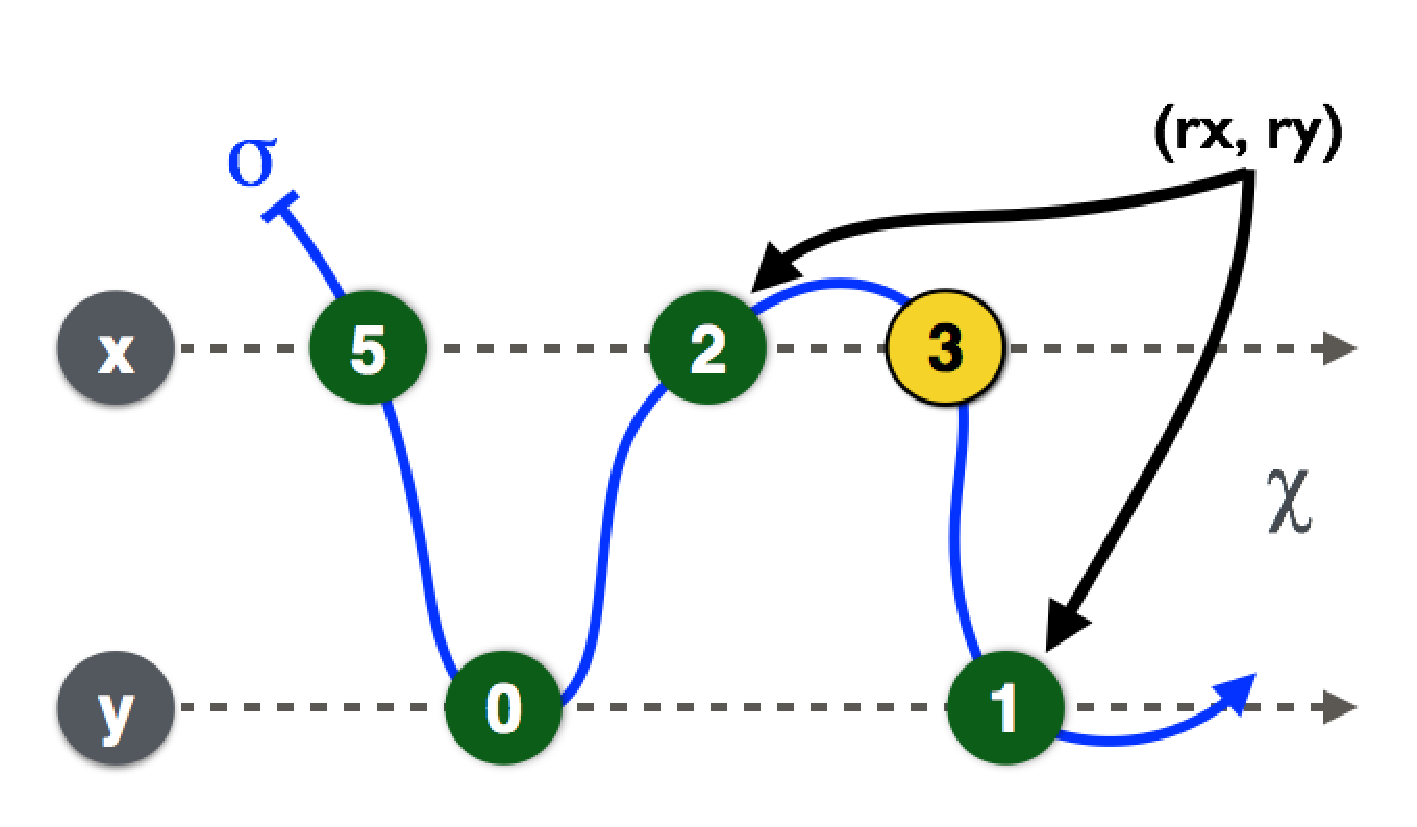
\includegraphics[width=6.1cm]{relink-before3.pdf}
\caption{\label{fig:reorder:before}} % Logical $=$ Real Time order, not a snapshot}
\end{subfigure} \hfill
\begin{subfigure}[t]{0.49\textwidth}
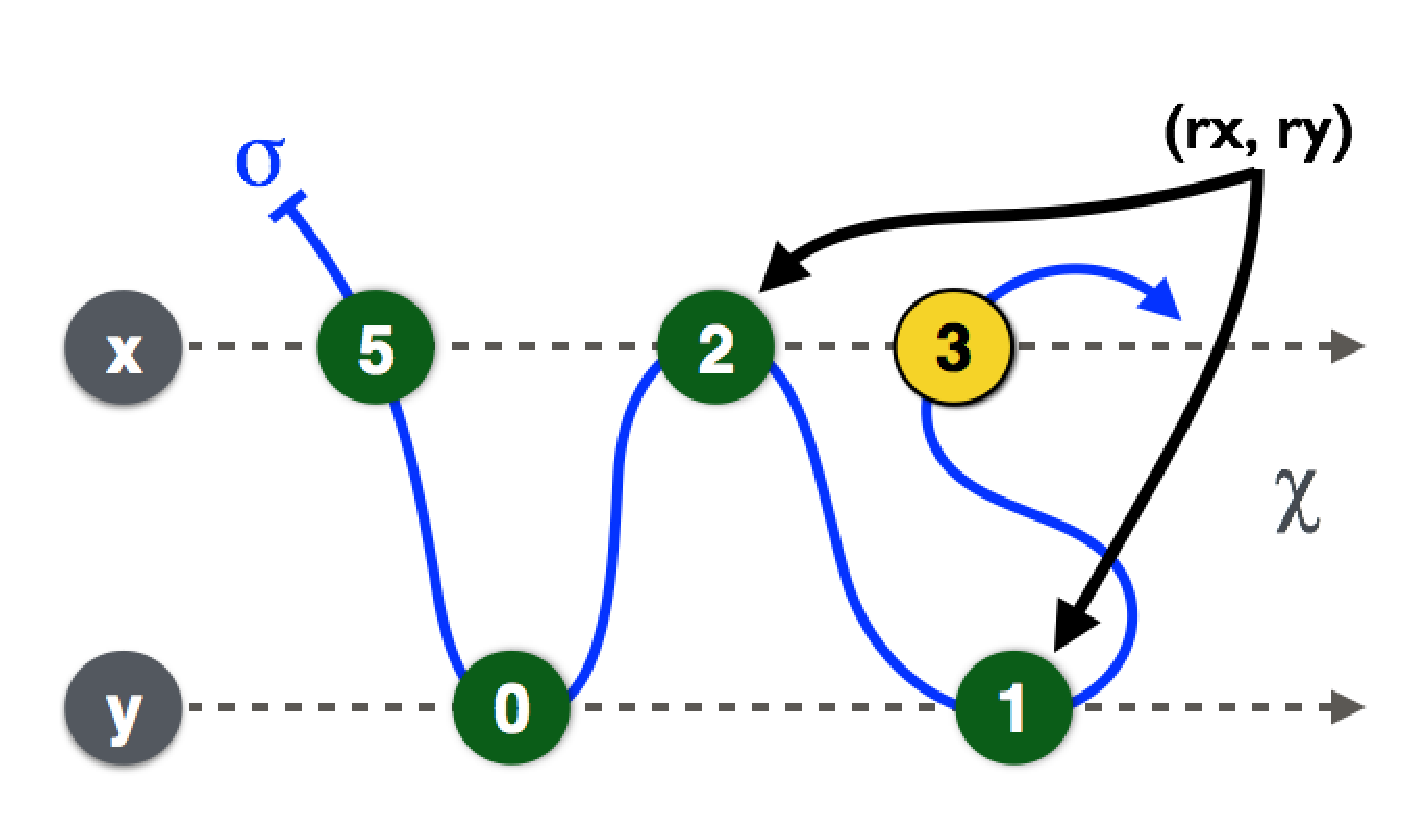
\includegraphics[width=6.1cm]{relink-after3.pdf}
\caption{\label{fig:reorder:after}} % Logical $\neq$ Real Time order, snapshot OK}
\end{subfigure}%
%
\caption{\label{fig:reorder} Changing the logical ordering (solid line
  $\ordlist$) of write events from (5, 0, 2, 3, 1) in
  (\subref{fig:reorder:before}) to (5, 0, 2, 1, 3) in
  (\subref{fig:reorder:after}), to reconcile with {\tt scan} returning
  the snapshot $\x=2, \y=1$, upon missing the write of $3$. Dashed
  lines $\hist$ represent real-time ordering.}
\end{figure}


Obviously, the high-level pattern of the proof requires tracking the
\emph{logical ordering} of the \jywrite\ and \jyscan\ events, which
differs from their \emph{real-time ordering}. As the logical ordering
is inherently dynamic, depending on properties such as
\jyscan\ missing a \jywrite, we formalize it in Hoare logic, by
keeping it as a list of events in auxiliary state that can be
dynamically reordered as needed. For example, Figure~\ref{fig:reorder}
shows the situation in the execution of \jyscan~that we reviewed
above. We start with the (initializing) writes of $5$ and $0$ already
executed, and our program performs the writes of $2$, $3$ and $1$ in
the real time order shown by the position of the events on the dashed
lines. In Figure~\ref{fig:reorder:before}, the logical order
$\ordlist$ coincides with real-time order, but is unsound for the
snapshot $\x=2, \y=1$ that \jyscan~wants to return. In that case, the
auxiliary code with which we annotate \jyscan, will change the
sequence $\ordlist$ in-place, as shown in
Figure~\ref{fig:reorder:after}.

Our specification and verification challenge then lies in reconciling
the following requirements. First, we have to posit specs that
say that \jywrite\ performs a write, and \jyscan\ performs a scan of
the memory, with the operations executing in a single logical
moment. Second, we need to implement the event reordering discipline
so that a method call only reorders events that overlap with it; the
logical order of the past events should be preserved. This will be
accomplished by introducing yet further structures into the auxiliary
state and code. Finally, the specs must hide the specifics of
the reordering discipline, which should be internal to the snapshot
object. Different snapshot implementations should be free to implement
different reorderings, without changing the method specs.


%Our challenge then lies in reconciling the following two conflicting
%requirements. First, we need to implement the reordering discipline so
%that the subsequent calls to \jywrite~and \jyscan~preserve the
%established logical order of the past events. This will be
%accomplished by introducing yet further structures into the auxiliary
%state and code. Second, we have to engineer Hoare triples for
%\jywrite~and \jyscan~to be \emph{intuitive} and \emph{helpful} to
%clients, but also to \emph{not expose} the specifics of the reordering
%discipline, which is internal to the snapshot object\footnotemark.
%%We discuss these issues next.
%\footnotetext{\ie we want to give the methods {\it principal} specifications}



\section{Background on FCSL}
\label{sec:background}

A Hoare specification in FCSL has the form
$\spec{P}\ e\ \spec{Q} @ \rcon$. $P$ and $Q$ are the precondition and
postcondition for $e$, and $\rcon$ defines the \emph{resource} on
which $e$ operates. We have elided $\rcon$ from the specs in
Section~\ref{sec:overview}, but explain it now. A resource is a state
transition system describing the state (real and auxiliary) and atomic
operations that the threads that want to simultaneously operate on
that state have to respect. For example, the state space
(aka.~resource invariants) of the resource $\cal E$ for the exchanger
is described by the predicates~\eqref{tag:exchanging} and
\ref{exP}--\ref{ex:gapless}. On the other hand, the transitions of
$\cal E$ can be read off from our discussion of the exchanger proof
outline, where at each atomic operation of \code{CAS}, we explicitly
described how the operation modifies the auxiliary state. These
modifications are the transitions that one has to declare in $\rcon$,
and then prove, when establishing $\spec{P}\ e\ \spec{Q} @ \rcon$,
that $e$ only makes declared transitions.

But a resource also has an important secondary role. Its definition
provides the variables that $P$ and $Q$ may scope over. For example,
in the case of exchanger, we used the variables $\heaps, \perms,
\hists$, $\heapo, \permo, \histo$, and $\heapj, \pending$.  Of course,
different resources will provide different state spaces, transitions
and variables. For example, a commonly used resource is $\cal P$ for
\emph{private state}. $\cal P$ allows only variables $\heaps$ and
$\heapo$ of type heap, denoting the private heap of a thread, and the
private heap of other threads. The transitions of $\cal P$ allow for
reading, writing, allocating and deallocating pointers from $\heaps$.

The mechanism by which a resource defines the allowed variables is as
follows. Underneath, a resource comes with only three variables:
$a_\lcl$, $a_\env$ and $a_\joint$ standing for abstract self state,
other state, and shared (joint) state, but the user can pick their
types depending on the application. In the case of $\cal E$, $a_\lcl$
and $a_\env$ are triples containing a heap, an offer-set and a
history. The variables we used in Section~\ref{sec:overview} are then
merely projections out of such triples:
$a_\lcl\,{=}\,(\heaps, \perms, \hists)$, and
$a_\env\,{=}\,(\heapo, \permo, \histo)$. Similarly,
$a_\joint\,{=}\,(\heapj, \pending)$.

It is essential that $a_\lcl$ and $a_\env$ have a common type, which
moreover, exhibits the algebraic structure of a \emph{partial
  commutative monoid} (PCM). A PCM requires a partial binary operation
$\bullet$ which is commutative and associative, and has a unit. In the
case of $\cal E$, each of the three components of $a_\lcl$ and
$a_\env$---heaps, offer-sets and histories---form a PCM, where
$\bullet$ is disjoint union $\hunion$, and $\emptyset$ is the
unit. Hence, the product of the three is a PCM as well, with $\bullet$
and unit defined point-wise. PCMs are important, as they give a way,
generic in $\rcon$, to define the inference rule for parallel composition.
%
\[
\tag{\normalsize \arabic{tags}}\refstepcounter{tags}\label{eq:parrule}
{\small{
\begin{array}{c}
\specK{\{P_1\}}\ e_1\ \specK{\{Q_1\}} @ \rcon \quad \specK{\{P_2\}}\ e_2\ \specK{\{Q_2\}} @ \rcon\\[2pt]
\hline\\[-7pt]
\specK{\{P_1 \circledast P_2\}}\ e_1 \parallel e_2\ \specK{\{[\res.1/\res]Q_1 \circledast [\res.2/\res]Q_2\}} @ \rcon
\end{array}
}}
\]
%
Here, $\circledast$ is defined as follows.
\[
\tag{\normalsize \arabic{tags}}\refstepcounter{tags}\label{eq:ssep}
\begin{array}{c}
(P_1 \circledast P_2)(a_\lcl, a_\joint, a_\env) \iff \exists x_1~x_2\ldot a_\lcl = x_1 \bullet x_2, \hbox{}\\
 P_1 (x_1, a_\joint, x_2 \bullet a_\env), P_2 (x_2, a_\joint, x_1 \bullet a_\env)
\end{array}
\]
%
%
The inference rule, and the definition of $\circledast$, formalize the
intuition that when a parent thread forks $e_1$ and $e_2$, then $e_1$
is part of the environment for $e_2$ and vice-versa. This is so
because the \emph{self} component $a_\lcl$ of the parent thread is
split into $x_1$ and $x_2$; $x_1$ and $x_2$ become the \emph{self}
parts of $e_1$, and $e_2$ respectively, but $x_2$ is also added to the
\emph{other} component $a_\env$ of $e_1$, and dually, $x_1$ is added
to the \emph{other} component of $e_2$.
%
Also note that parallel composition returns a pair of the outputs
produced by $e_1$ and $e_2$. Thus, the variable $\res$ in $Q_1$ and
$Q_2$ has to be appropriately renamed by the projections $\res.1$ and
$\res.2$ in the postcondition of the parallel composition.

The rule of frame of FCSL is a special case of parallel composition,
when $e_2$ is the idle thread.
%
\[
\tag{\normalsize \arabic{tags}}\refstepcounter{tags}\label{eq:frame}
{\small{
\begin{array}{c}
\specK{\{P_1\}}\ e\ \specK{\{P_2\}} @ \rcon\\[2pt]
\hline\\[-7pt]
\specK{\{P_1 \circledast Q\}}\ e\ \specK{\{P_1 \circledast Q\}} @ \rcon
\end{array}\qquad 
\begin{array}{c}
\mbox{$Q$ stable under}\\
\mbox{$\rcon$'s transitions}
\end{array}
}}
\]
A notable difference from the frame rules of other separation logics
is that FCSL's definition of $\circledast$ forces that the value being
framed onto \emph{self} component is \emph{subtracted} from the
\emph{other} component, whereas in other separation logic, the frame
value materializes out of nowhere. To illustrate, we can frame
$\gists$ onto the history $\hists$ in the the
spec~(\ref{tag:exchangespec}), by taking
$\rcon\,{\eqdef}\,a_\lcl\,{=}\,(\heaps, \hists,
\perms)\,{=}\,(\emptyset, \gists, \emptyset)$.
We obtain, after some simplification:
%
\[
{\small{
\begin{array}{c}
\specK{\{\heaps = \emptyset, \perms = \emptyset, \hists = \gists, \gist \subseteq \gists \hunion \histo \hunion \mygather{\pending}\}}\\[2pt]
\mathtt{exchange}\ v \\[2pt]
\spec{\!\!
  \begin{array}{c}
    \heaps = \emptyset, \perms = \emptyset, \gist \subseteq \gists \hunion \histo \hunion \mygather{\pending}, \hbox{}\\[1pt]
    \mathsf{if}\ \res\ \mathsf{is}\ \mathsf{Some}\ w\ \mathsf{then}\\[1pt]
    \exists t\ldot \hists = t \mapsto (v, w) \hunion \gists, 
    \mathsf{last} (\gist) < t, \twin{t}~\mathsf{else}\ \hists = \gists    
  \end{array}
\!\!}@\cal E
\end{array}
}}
\]
But notice how the spec now says that $\gist \subseteq \gists \hunion
\histo \hunion \mygather{\pending}$, whereas
in~(\ref{tag:exchangespec}) it said $\gist \subseteq \histo \hunion
\mygather{\pending}$. The addition of $\gists$ compensates for
$\gists$ having been subtracted out of $\histo$, to be moved to
$\hists$.

Finally, we will use one more constructor of FCSL, and its associated
inference rule: \emph{hiding}. The program $\mathsf{hide}\ e$
operationally just executes $e$, but logically allows installing a
resource within the scope of $e$. For example, a program can start
only with private heap variables $\heaps$ and $\heapo$ (\ie, using
only the resource $\cal P$). However, it can then take a chunk of heap
out of $\heaps$ and ``install'', for instance, an exchanger resource
$\cal E$ in it, thereby giving the threads in $e$ the ability to
exchange values. The spec of $e$ is then expressed using the variables
that $\cal E$ adds to $\cal P$: $\perms, \hists$, $\permo, \histo$,
and $\heapj, \pending$. Upon termination, the extra variables are
removed from the scope. We elide here the general form of the hiding
rule (it is given in~\cite{Nanevski-al:ESOP14}), and just provide the
special case involving $\cal E$ and $\cal P$.
\[
\tag{\normalsize \arabic{tags}}\refstepcounter{tags}\label{eq:ehide}
{\small{
\begin{array}{c}
\specK{\{P\}}\ e\ \specK{\{Q\}} @ \cal E\\[2pt]
\hline\\[-7pt]
\specK{\{\heaps = \Phi_1(\heapj), \Phi_1(P)\}}\ \mathsf{hide}_{\Phi_1}~e\ \specK{\{\exists \Phi_2\ldot \heaps = \Phi_2(\heapj), \Phi_2(Q)\}} @ \cal P
\end{array}
}}
\]
When read bottom up, the rule says that we can install the resource
$\cal E$ in the scope of a thread that works with $\cal P$, but then
we need substitutions $\Phi_1$ and $\Phi_2$, to map variables of $\cal
E$ ($\heaps, \perms, \hists$, \etc) to values expressed with variables
from $\cal P$ ($\heaps$, and $\heapo$). Here $\Phi_1$ is an initial
such substitution (user provided), and the rule guarantees the
existence of an ending substitution $\Phi_2$. The substitutions have
to satisfy a number of side conditions, which we elide here for
brevity. The most important one is that $\Phi_1$, $\Phi_2$, fix the
\emph{other} variable $a_\env = (\heapo, \permo, \histo)$ to be the
PCM unit (\ie,~a triple of empty sets). Fixing $a_\env$ to unit
formalizes the intuition that within the scope of $\mathsf{hide}$,
the outside threads cannot see $\cal E$, and thus cannot interfere
with the exchanges performed by $e$. They start with empty heap,
offer-set and history, and terminate with empty ones too.

At the beginning of $\mathsf{hide}~e$, the private heap equals the
value that $\Phi_1$ gives to $\heapj$ ($\heaps = \Phi_1(\heapj)$). In
other words, the $\mathsf{hide}$ rule takes the private heap of a
thread, and makes it shared, \ie, gives it to the $\heapj$ component
of $\cal E$. Upon finishing, $\mathsf{hide}~e$ makes $\heapj$ private
again.
%
%($\heaps = \Phi_2(\heapj)$).

%\an{Should I say something about compositionality? Why is FCSL
%  compositional? Maybe say, soundness of FCSL has been established by
%  shallow embeding in Coq. Thus, the logic immediately inherits the
%  substitution principle, thereby allowing that clients can reason
%  only out of the Hoare spec of an object.}

%\subsection{FCSL basics}
%\label{sec:fcsl-basics}
%
%\todo{A short overview of FCSL: mostly, concerning subjectivity and hiding}
%
%\subsection{Histories as auxiliary state}
%\label{sec:hist-state} 


\section{Verifying Exchanger's Client}
\label{sec:cal}
\newcommand{\ts}{{ts}}
\newcommand{\vvs}{{vs}}
\newcommand{\acc}{{ac}}
\newcommand{\ws}{{ws}}
\newcommand{\sorted}[1]{\mathsf{sorted}\ #1}

%\paragraph{Client definition.}
We next illustrate how the verified exchanger from
Section~\ref{sec:overview} can be used by client programs, and how the
\emph{other} component, asserted by the spec to satisfy $\gist
\subseteq \histo \hunion \mygather{\pending}$, is crucial in this
process.
%
We emphasize that proof of the client does not see the fine-grained
implementation details of the exchanger, which are hidden by
spec~\eqref{tag:exchangespec}.
%
A version of the client we consider is actually used in
\code{java.util.concurrent}~\cite{ExchangerClass}, and is defined as
follows. First, we make the exchanger loop until it succeeds in
exchanging the value.
%
\vspace{-5pt}
\[
\vspace{-5pt}
{\small{
\begin{array}{rl}
& \esc{exchange'}~(v : A) : A = \{\\[1pt]
&  ~~~~ w' \Asgn \esc{exchange}~v;\\[1pt]
&  ~~~~
  \kw{if}~~w'~~\kw{is}~~\esc{Some}~w~~\kw{then}~~\kw{return}~w~~\kw{else}~~\esc{exchange'}~v~\}
\end{array}
}}
\]
%
Next, $\esc{exchange'}$ is iterated over a sequence, exchanging each
element in order, appending the received matches to an accumulator. 
%
\vspace{-5pt}
\[
\vspace{-5pt}
{\small{
\begin{array}{rl}
& \esc{ex\_seq}~(\vvs, \acc : \esc{seq}~A) : \esc{seq}~A = \{\\[1pt]
& ~~~~ \kw{if}~~\vvs~~\kw{is}~~v{::}\vvs'~~\kw{then}\\[1pt]
& ~~~~ ~~~~ w \Asgn \esc{exchange'}~v;~~\esc{ex\_seq}~(\vvs', \esc{snoc}~\acc~w)\\[1pt]
& ~~~~ \kw{else}~~\kw{return}~\acc~\}
\end{array}
}}
\]
%
Our goal is to show
% compositionally, \ie~reasoning only out of the
%spec of $\mathtt{exchange}$, 
that the parallel composition
%
\[
e = \esc{ex\_seq}~(\vvs_1, \esc{nil}) \parallel \esc{ex\_seq}~(\vvs_2, \esc{nil})
\]
%
exchanges $\vvs_1$ and $\vvs_2$, \ie,~returns the pair $(\vvs_2,
\vvs_1)$. This is a valid property, assuming that $e$ runs without
interference, so that the two threads in $e$ have no choice but to
exchange the values between themselves. We make the assumption
explicit by using the $\hide$ constructor. Thus, the Hoare
triple we will prove is:
%
\[
\tag{\arabic{tags}}\refstepcounter{tags}\label{tag:hidespec} 
{\small{
\!\!\!
\begin{array}{c}
\specK{\{\heaps = g \mapsto\mathsf{null}\}}~~\hide~~e~~\specK{\{g \in
  \mathsf{dom}~\heaps, \res = (\vvs_2, \vvs_1)\}} @ \cal P
\end{array}
}}
\]
%
It says that we start with a heap where $g$ stores $\mathsf{null}$,
and end with a possibly larger heap (due to the memory leak of the
exchanger), but with the result $\res = (\vvs_2, \vvs_1)$.

%$vs$ and $ws$ are exchanged. This is a valid property under the
%assumptions that the two $\esc{ex\_seq}$ threads run in isolation,
%\ie, without interfernce from any other exchanging threads. In that
%case, the two threads have no other options but to exchange values
%between themselves.

\paragraph{Explaining the verification.}
%
The proof of $\hide~~e$ involves several stages: verification of
$\esc{exchange'}$, $\esc{ex\_seq}$, $e$ and finally $\hide~e$. We only
list the specs involved in the first two stages, omitting the
associated proof outlines. These are straightforward, as the programs
contain only sequential composition, and can be found in our Coq
scripts. The last two stages employ parallel composition and $\hide$,
and are thus more involved, so we present them in detail.

The following are the specs for $\esc{exchange'}$ and $\esc{ex\_seq}$.
%
\[
{\small{
\begin{array}{c}
\specK{\{\heaps = \emptyset, \perms = \emptyset, \hists = \gists, \gist \subseteq \gists \hunion \histo \hunion \mygather{\pending}\}}\\[2pt]
\esc{exchange'}\ v\\[2pt]
\spec{\!\!
\begin{array}{c}
\heaps = \emptyset, \perms = \emptyset, \gist \subseteq \gists \hunion
  \histo \hunion \mygather{\pending}, \\[1pt]    
\exists t\ldot \hists = t \mapsto (v, \res) \hunion \gists, \mathsf{last} (\gist) < t, \twin{t}
\end{array}
\!\!}@\cal E
% \specK{\{\heaps = \emptyset, \perms = \emptyset, \gist \subseteq \gists \hunion \histo \hunion \mygather{\pending}, \hbox{}}\\
% \specK{\exists t\ldot \hists = t \mapsto (v, \res) \hunion \gists, \mathsf{last} (\gist) < t, \twin{t}\}} @ 
\end{array}
}}
\]
%
%\vspace{-10pt}
%
\[
{\small{
\!\!\!
\begin{array}{c}
\spec{\!\!
\begin{array}{c}
\heaps = \emptyset, \perms = \emptyset, \hists = \mathsf{zip}~\ts~\vvs~\acc, \hbox{}\\[1pt]
\sorted{\ts}, \mathsf{zip}~\overline{\ts}~\acc~\vvs \subseteq \histo \hunion \mygather{\pending}
\end{array}
\!\!}
\\[2pt]
\mathtt{ex\_seq}~\vvs'~\acc\\[2pt]
\spec{\!\!\!\!
\begin{array}{c}
\exists \ts'~\acc'\ldot\heaps = \emptyset, \perms = \emptyset, \res =
  \acc~\esc{++}~\acc',\\[1pt] 
\hists = \mathsf{zip}~(\ts~\esc{++}~\ts')~(\vvs~\esc{++}~\vvs')~(\acc~\esc{++}~\acc'), 
 \sorted{(\ts~\esc{++}~\ts')},\\[1pt]
\mathsf{zip}~(\overline{\ts}~\esc{++}~\overline{\ts'})~(\acc~\esc{++}~\acc')~(\vvs~\esc{++}~\vvs') \subseteq 
      \histo  \hunion \mygather{\pending}
\end{array}
\!\!\!\!}@\cal E
\end{array}
}}
\]

The spec for $\esc{exchange'}$ is immediately derived
from~(\ref{tag:exchangespec}) by removing the now-impossible case of
exchange failing, and then framing the history components by $\gists$,
as explained in Section~\ref{sec:background}.
%
The spec for $\esc{ex\_seq}$ is more complicated.  It starts with two
logical variables $\ts$ and $\vvs$. The conjunct
$\hists = \mathsf{zip}~\ts~\vvs~\acc$ in the precondition says that
$\ts$ is the list of time-stamps currently generated by our thread,
and $\vvs$ is the list of values exchanged for those in $\acc$. Here
$\mathsf{zip}$ creates a history out of a list of time-stamps and
values:
%
\[
{\small{
\mathsf{zip}~ts~vs~ws = \left\{%
\begin{array}{l}
t \mapsto (v, w) \hunion \mathsf{zip}~\ts'~\vvs'~\ws', \\
\hphantom{\emptyset,}\ \mbox{if $\ts=t\,{::}\,\ts', \vvs=v\,{::}\,\vvs', \ws=w\,{::}\,\ws'$}\\
\emptyset, \mbox{if $\ts = \vvs = \ws = \mathsf{nil}$}\\
\mbox{undefined}, \mbox{otherwise}
\end{array}\right.
}}
\]
%
%\[
%\begin{array}{c}
%\mathsf{zip}~(t\,{::}\,ts)~(v\,{::}\,vs)~(w\,{::}\,ws) = 
%  t \mapsto (v, w) \hunion \mathsf{zip}~ts~vs~ws\\
%\mathsf{zip}~\mathsf{nil}~\mathsf{nil}~\mathsf{nil} = \emptyset\\
%\mathsf{zip}~ts~vs~ws = \mbox{undefined otherwise}
%\end{array}
%\]
The precondition further assumes that the time-stamps in $\ts$, when
considered as natural numbers, strictly grow ($\sorted{\ts}$), and
that the \emph{other} history contains the ``twin'' history of
$\hists$: $\mathsf{zip}~\overline{\ts}~\acc~\vvs \subseteq \histo
\hunion \mygather{\pending}$. Here $\overline{\ts}$ denotes the list
of twin time-stamps of $\ts$, and $\acc$ and $\vvs$ appear in the
reversed order compared to $\hists$.

The postcondition says that $\esc{ex\_seq}$ adds a list of time-stamps
$\ts'$, which are all larger than time-stamps in $\ts$ and also
strictly grow. Intuitively, this holds because the postcondition of
$\esc{exchange'}$ ensures the time-stamp $t$ is larger than any
time-stamps used in $\hists$, $\histo$ or $\pending$ (by choosing the
logical variable $\gist$ in the spec of $\esc{exchange'}$ to be the
union of $\hists$, $\histo$ and $\mygather{\pending}$). The self
history $\hists$ is extended with the new time-stamps and values:
$\hists =
\mathsf{zip}~(\ts~\esc{++}~\ts')~(\vvs~\esc{++}~\vvs')~(\acc~\esc{++}~\acc')$. Similarly
for the environment history, which must be a twin of $\hists$ by the
resource invariant~(\ref{tag:exchanging}). The result $\res$ appends
an unknown list of values $\acc'$, supplied by interfering threads, to
the starting list $\acc$.

The above spec for $\esc{ex\_seq}$ is also used as its loop
invariant. For use in clients, we restrict it to
$\acc = \ts = \vvs = \mathsf{nil}$, and derive:
%
\[
{\small{
\begin{array}{c}
\specK{\{\heaps = \emptyset, \perms = \emptyset, \hists = \emptyset\}}\\[2pt]
\mathtt{ex\_seq}~vs~\mathsf{nil}\\[2pt]
\spec{\!\!\!
\begin{array}{c}
\exists \ts\ldot \heaps = \emptyset, \perms = \emptyset, 
\mathsf{sorted}~\ts, \hists = \mathsf{zip}~\ts~\vvs~\res,
\\[1pt]
\mathsf{zip}~\overline{\ts}~\res~\vvs \subseteq \histo  \hunion \mygather{\pending}  
\end{array}
\!\!\!}@ \cal E
\end{array}
}}
\]
%
Naming the postcondition above as $Q(\vvs)$, we can now verify the
parallel composition $e$.
%
\[
\tag{\arabic{tags}}\refstepcounter{tags}\label{tag:e}\\
{\small{
\begin{array}{c}
\specK{\{\heaps = \emptyset, \perms = \emptyset, \hists = \emptyset\}}\\[2pt]
%\specK{\{\heaps = \emptyset\hunion\emptyset, \perms = \emptyset\hunion\emptyset, \hists = \emptyset\hunion\emptyset\}}\\
\specK{\{(\heaps = \emptyset, \perms = \emptyset, \hists = \emptyset) \circledast 
  (\heaps = \emptyset, \perms = \emptyset, \hists = \emptyset)\}}\\[2pt]
\begin{array}{c}
\specK{\{\heaps = \emptyset, \perms = \emptyset, \hists = \emptyset\}}\\[1pt]
\mathsf{ex\_seq}~\vvs_1~\mathsf{nil}\\[1pt]
\specK{\{Q(\vvs_1)\}}
\end{array} \parallel
\begin{array}{c}
\specK{\{\heaps = \emptyset, \perms = \emptyset, \hists = \emptyset\}}\\[1pt]
\mathsf{ex\_seq}~\vvs_2~\mathsf{nil}\\[1pt]
\specK{\{Q(\vvs_2)\}}
\end{array}\\[2pt]
\specK{\{Q(\vvs_1) \circledast Q(\vvs_2)\}}\makebox[0pt]{\quad $@ \cal E$}
\end{array}
}}
\]
Unfolding the definition of $\circledast$, the postcondition obtains:
%
%{\small{
\begin{align*}
\exists \ts_1~& \ts_2\ldot \heaps = \emptyset, \perms = \emptyset, \mathsf{sorted}~{\ts_1}, \mathsf{sorted}~{\ts_2},\\
& \hists = \mathsf{zip}~\ts_1~\vvs_1~\res.1 \hunion \mathsf{zip}~\ts_2~\vvs_2~\res.2,\\
& \mathsf{zip}~\overline{\ts_1}~\res.1~\vvs_1 \subseteq \mathsf{zip}~\ts_2~\vvs_2~\res.2 \hunion \histo \hunion\mygather{\pending}, \tag{\arabic{tags}}\refstepcounter{tags}\label{tag:x}\\
& \mathsf{zip}~\overline{\ts_2}~\res.2~\vvs_2 \subseteq \mathsf{zip}~\ts_1~\vvs_1~\res.1 \hunion \histo \hunion\mygather{\pending}. \tag{\arabic{tags}}\refstepcounter{tags}\label{tag:y}
\end{align*}
%}}
%
Intuitively, the values of each \emph{self} component $\heaps$,
$\perms$, $\hists$ from $Q(\vvs_1)$ and $Q(\vvs_2)$ are joined into
the self component of the joined thread. At the same time, the
\emph{other} component $\histo$ of the left thread equals the sum of
the $\hists$ of the right thread, and the $\histo$ of the joining
thread. Thus, the predicates $\mathsf{zip}~\overline{\ts}~\res~\vvs
\subseteq \histo \hunion \mygather{\pending}$ from $Q_1$ and $Q_2$
become $(\ref{tag:x})$ and $(\ref{tag:y})$, respectively.
%\[
%\begin{array}{c}
%\{\heaps = \emptyset, \perms = \emptyset, \chi_s = \emptyset\}\\
%\{\heaps = \emptyset\hunion\emptyset, \perms = \emptyset\hunion\emptyset, \chi_s = \emptyset\hunion\emptyset\}\\
%\begin{array}{c}
%\{\heaps = \emptyset, \perms = \emptyset, \chi_s = \emptyset\}\\
%\mathsf{ex\_seq}~vs_1~\mathsf{nil}\\
%\{\heaps = \emptyset, \perms = \emptyset, \\
%\exists ts_1\ldot \mathsf{sorted}~ts_1, \\
%  \chi_s = \mathsf{zip}~ts_1~vs_1~\res, \\
% \mathsf{zip}~\overline{ts_1}~\res~vs_1 \subseteq \chi_o \hunion \mygather{\pending}\}
%\end{array} \parallel
%\begin{array}{c}
%\{\heaps = \emptyset, \perms = \emptyset, \chi_s = \emptyset\}\\
%\mathsf{ex\_seq}~vs_2~\mathsf{nil}\\
%\{\heaps = \emptyset, \perms = \emptyset, \\
%\exists ts_2\ldot \mathsf{sorted}~ts_2, \\
%  \chi_s = \mathsf{zip}~ts_2~vs_2~\res, \\
%\mathsf{zip}~\overline{ts_2}~\res~vs_2 \subseteq \chi_o \hunion \mygather{\pending}\}
%\end{array}\\
%\{\heaps = \emptyset, \perms = \emptyset, \exists ts_1~ts_2\ldot \mathsf{sorted}~ts_1, \mathsf{sorted}~ts_2,\\
%\chi_s = \mathsf{zip}~ts_1~vs_1~\res.1 \hunion \mathsf{zip}~ts_2~vs_2~\res.2\\
%\mathsf{zip}~\overline{ts_1}~\res.1~vs_1 \subseteq \mathsf{zip}~ts_2~vs_2~\res.2 \hunion \chi_o \hunion\mygather{\pending}\\
%\mathsf{zip}~\overline{ts_2}~\res.2~vs_2 \subseteq \mathsf{zip}~ts_1~vs_1~\res.1 \hunion \chi_o \hunion\mygather{\pending}\}
%\end{array}
%\]

What does this postcondition say? First, the self history of $e$
contains both $\mathsf{zip}~\ts_1~\vvs_1~\res.1$ and
$\mathsf{zip}~\ts_2~\vvs_2~\res.2$. Thus, $\vvs_1$ is exchanged for
$\res.1$, and $\vvs_2$ for $\res.2$. But we additionally want to
conclude that $\res.1 = \vvs_2$ and $\res.2 = \vvs_1$, \ie, the lists
are exchanged for each other, in the absence of interference.

To derive this desired property, we will use the inequalities
$(\ref{tag:x})$ and $(\ref{tag:y})$. Notice that $(\ref{tag:x})$ and
$(\ref{tag:y})$ are ultimately instances of the conjunct
$\gist \subseteq \histo \hunion \mygather{\pending}$ that was part of
the specification~(\ref{tag:exchangespec}). Hence, this example
justifies the use of subjectivity in specs.

First, we apply $\hide$ to the spec~$(\ref{tag:e})$, to limit the
interference on $e$. We pick substitution
$\Phi_1 = [\emptyset/\heaps, \emptyset/\perms, \emptyset/\hists,
g\,{\mapsto}\,\mathsf{null}/\heapj$,
$\emptyset/\pending, \emptyset/\heapo, \emptyset/\permo,
\emptyset/\histo]$,
and obtain (via the $\hide$ rule~\eqref{eq:ehide}):
%
\[
{\small{
\begin{array}{c}
\specK{\{\heaps = g \mapsto \mathsf{null}\}}\\[2pt]
\specK{\{\heaps = g \mapsto \mathsf{null}, \Phi_1 (\heaps = \emptyset, \perms = \emptyset, \hists = \emptyset)\}}\\[2pt]
\hide_{\Phi_1}~~e \\[2pt]
\specK{\{\exists \Phi_2\ldot \heaps = \Phi_2(\heapj), \Phi_2(Q (\vvs_1) \circledast Q(\vvs_2))\}} @ \cal P
\end{array}
}}
\]
%
From the unfolding of $Q(\vvs_1) \circledast Q(\vvs_2)$, we obtain
that $\Phi_2$ must be such that $\heaps$ and $\perms$ map to
$\emptyset$, and $\hists$ maps to $\mathsf{zip}~\ts_1~\vvs_1~\res.1
\hunion \mathsf{zip}~\ts_2~\vvs_2~\res.2$. Moreover, by the general
conditions on $\Phi$, $\permo$ and $\histo$ also map to
$\emptyset$. The variable $\heapj$ maps to some heap which, by
resource invariant~\ref{exP}, must contain the pointer $g$. Hence,
from $\heaps = \Phi_2(\heapj)$, we derive $g \in
\mathsf{dom}~\heaps$. Also by resource invariant~\ref{matched},
$\mathsf{dom}\ \pending = \perms \hunion \permo$, and thus $\pending$
too must map to $\emptyset$. Hence, we can weaken and simplify the
postcondition into:
\begin{align*}
\exists \ts_1~\ts_2\ldot & g \in \mathsf{dom}\ \heaps, \sorted{\ts_1}, \sorted{\ts_2}\\
& \mathsf{zip}~\overline{\ts_1}~\res.1~\vvs_1 \subseteq \mathsf{zip}~\ts_2~\vvs_2~\res.2 \tag{\ref{tag:x}'}\label{tag:x'}\\
& \mathsf{zip}~\overline{\ts_2}~\res.2~\vvs_2 \subseteq \mathsf{zip}~\ts_1~\vvs_1~\res.1 \tag{\ref{tag:y}'}\label{tag:y'}
\end{align*}
%
Now, histories are finite maps from time-stamps to value pairs. Hence
$(\ref{tag:x'})$ implies that the time-stamps from $\overline{\ts_1}$
are included in the time-stamps of $\ts_2$. Similarly from
$(\ref{tag:y'})$, $\overline{\ts_2}$ is included in $\ts_1$. Thus,
$\ts_1$ and $\ts_2$ are of same size, and moreover, since they both
are strictly increasing, it must be that $\ts_2 =
\overline{\ts_1}$. Therefore, $(\ref{tag:x'})$ can be strengthened
into an equality: 
%
\[
\mathsf{zip}~\overline{\ts_1}~\res.1~\vvs_1 = \mathsf{zip}~\ts_2~\vvs_2~\res.2
\]
%
As the time-stamps in $\overline{\ts_1}$ and $\ts_2$ appear
in the same order, it must be $\res.1 = \vvs_2$ and $\vvs_1 = \res.2$,
leading to the desired (\ref{tag:hidespec}).  
%
% \an{I omitted here some steps. In particular, that $\sorted{\ts_1}$
%   implies $\sorted{\overline{\ts_1}}$ is not straightforward, and
%   requires also deriving that there are no twins in $\ts_1$. That can
%   all been done (and has been done), but should we present it?}




\section{Specifying Counting Networks}
\label{sec:counting}

We now show how to use subjective histories to specify another class
of non-linearizable objects---\emph{counting networks}.
%
Counting networks are a special case of \emph{balancing networks}
introduced by Aspnes \etal~\cite{Aspnes-al:JACM94}, themselves
building on sorting networks~\cite{Ajtai-al:STOC83}, aimed to
implement concurrent counters in a way free from synchronization
bottlenecks.
%
The key idea is to decompose the workload between \emph{several}
counters, so that each of them is responsible for a disjoint set of
values. A thread trying to increment first approaches the
\emph{balancer}, which is a logical ``switch'' that ``directs'' the
thread, \ie, provides it with the address of the counter to increment.
%
The balancers make counting networks' operations
\emph{non-linearizable}, as in the presence of interference the
results of increments might be observed out of order.
%
% \wrt~a sequential specification.
{
%\setlength{\belowcaptionskip}{-15pt} 
\begin{figure}%[18]{r}{4cm} 
\begin{tabular}{c@{\ \ \ \ \ \ }c}
\begin{minipage}[c]{2.5cm}
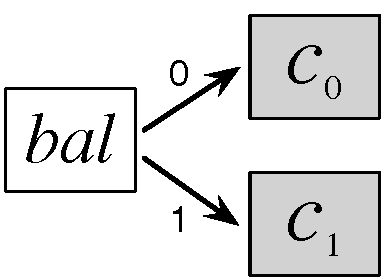
\includegraphics[width=2.1cm]{counter.pdf} 
\end{minipage}
&
\begin{minipage}[l]{4.9cm}
\centering
{\small{
\[
\begin{array}{rl}
\Num{1} & \esc{getAndInc()} : \esc{nat}~=~\esc{\{}  \\[2pt] 
\Num{2} & ~~~~ b \Asgn \esc{flip(}\bal\esc{)};\\[2pt]
\Num{3} & ~~~~ \res \Asgn \esc{fetchAndAdd2(}c_b\esc{)};\\[2pt]
\Num{4} & ~~~~ \kw{return}~\res~\esc{\}}
\end{array}
\]
}}
\end{minipage} 
%
\end{tabular}
%
\vspace{-10pt}  
\caption{Simple counting network}
\label{fig:counter-fig} 
%\vspace{-15pt}  
\end{figure}
}

Figure~\ref{fig:counter-fig} presents a schematic outline and a
pseudo-code implementation of a counting network with a single
balancer.
%
The implementation contains three pointers: the balancer $\bal$, which
stores either 0 or 1, thus directing threads to the shared pointers
$c_0$ or $c_1$, which count the even and odd values,
respectively. Threads increment by calling \code{getAndInc}, which
works as follows. It first atomically changes the bit value of the
balancer via a call to atomic operation \code{flip} (line 2). The
\code{flip} operation returns the \emph{previous} value $b$ of the
balancer as a result, thus determining which of the counters, $c_0$ or
$c_1$, should be incremented. The thread proceeds to atomically add 2
to the value of $c_b$ via \code{fetchAndAdd2} (line 3). The old value
of $c_b$ is returned as the result of the procedure.\footnote{In the
  counting network from Figure~\ref{fig:counter-fig}, the balancer
  itself might seem like a contention point. However, the \code{flip}
  operation is much less expensive than \code{CAS} as a
  synchronization mechanism. The performance can be further improved
  by constructing a \emph{diffracting tree} of several
  balancers~\cite[\S 12.6]{Herlihy-Shavit:08}, but we do not consider
  diffracting trees here.}

Assuming that $c_0$ and $c_1$ are initialized with $0$ and $1$, it is
easy to see that in a single-threaded program, the network will behave
as a conventional counter; that is, consecutive invocations of
\code{getAndInc} return consecutive nats.
%
However, in the concurrent setting, \code{getAndInc} may return
results out of order, as follows. 
%
% which historically led to the definition of quiescent
% consistency~\cite[\S 3.3]{Herlihy-Shavit:08} in order to specify the
% network's concurrent behavior.

\vspace{3pt}
\begin{example}
\label{ex:t1t2}
%
Consider two threads, $T_1$ and $T_2$ operating on the network
initialized with $\bal\,{\mapsto}\,0$, $c_b\,{\mapsto}\,b$. $T_1$
calls \code{getAndInc} and executes its line~2 to set $\bal$ to 1. It
gets suspended, so $T_2$ proceeds to execute lines~2 and~3, therefore
setting $\bal$ back to $0$ and returning $1$. While $T_1$ is still
suspended, $T_2$ calls \code{getAndInc} again, gets directed to $c_0$,
and returns 0, after it has just returned 1.
%
\end{example}
\vspace{3pt}

\noindent

This out-of-order behavior, however, is not random, and can be
precisely characterized as a function of the number of threads
operating on the
network~\cite{Afek-al:OPODIS10,Jagadeesan-Riely:ICALP14}. In the rest
of this section and in Section~\ref{sec:qclients}, we show how to
capture such bounds in the spec using auxiliary state of (subjective)
histories in a client-sensitive manner. As a form of road map, we list
the desired requirements for the spec of \code{getAndInc},
%
adapting the design goals of the criteria, such as QC, QQC and
QL~\cite{Aspnes-al:JACM94,Afek-al:OPODIS10,Jagadeesan-Riely:ICALP14},
which we will proceed to verify formally, following \textbf{\emph{Step
    1}} and \textbf{\emph{Step 2}} of our approach, and then employ in
client-side reasoning via \textbf{\emph{Step 3}}:
%
\vspace{2pt}
\begin{itemize}

\item \textbf{R1:} Two different calls to \code{getAndInc}
  should return distinct results (\emph{strong concurrent
    counter semantics}).

\item \textbf{R2:} The results of calls to \code{getAndInc},
  separated by a period of quiescence (\ie, absence of interference),
  should appear in their sequential order (\emph{quiescent
    consistency}).

\item \textbf{R3:} The results of two sequential calls $C_1$ and
  $C_2$, in a single thread should be out of order by no more than $2\
  N$, where $N$ is the number of interfering calls that overlap with
  $C_1$ and $C_2$ (\emph{quantitative quiescent consistency}).
%\an{Can we chose one of the two here: either qqc or ql?}

\end{itemize}

%\vspace{2pt}
%\lipsum[1]

\subsection{Step 1: counting network's histories and invariants}
\label{sec:counting-intuition}

To formalize the necessary invariants, we elaborate the counting
network with auxiliary state: \emph{tokens} (isomorphic to nats) and
novel \emph{interference-capturing histories}.

A \emph{token} provides a thread that owns it with the right to
increment an appropriate counter~\cite{Aspnes-al:JACM94}. In our
example, a thread that performs the \code{flip} in line 2 of
\code{getAndInc} will be awarded a token which it can then spend to
execute \code{fetchAndAdd2}.
%
Thus, any individual token represents a ``pending'' call to
\code{getAndInc}, and the set of unspent tokens serves as a bound on
the out-of-order behavior that the network exhibits. We introduce
auxiliary variables for the held tokens: $\tkns$ keeps the tokens
owned by the \emph{self} thread, with its \emph{even} and \emph{odd}
projections $\tkns^0$ and $\tkns^1$, such that $\tkns = \tkns^0
\hunion \tkns^1$, administering access to $c_0$ and $c_1$,
respectively. Similarly, $\tkno$, featuring the same projections,
keeps the tokens owned by the \emph{other} thread.  We abbreviate
$\tkn^i = \tkns^i \hunion \tkno^i$ for $i=0,1$.  
%
% \an{Is there a way to compute tokens out of some global
%   \emph{ordinary} history, so that we don't have to use an
%   \emph{interference-capturing} one? If not, we should stress the
%   point.}
%
% \is{I don't think there is, and I'm not sure if we have to elalorate
%   on this point.}

Figure~\ref{fig:chist} illustrates a network with three \emph{even}
tokens: $x^0, y^0, z^0 \in \tkn^0$, held by threads that will
increment $c_0$, and one \emph{odd} token $u^1 \in \tkn^1$, whose
owner will increment $c_1$.
%
%\an{Removed: We also point out here that token names (and their
%  uniqueness) will be of critical importance for the specifications we
%  give further. This point was never emphasized later on, so why
%  bother drawing attention to it.}

A \emph{history} of the counting network is an auxiliary finite map,
consisting of entries of the form $t \mapsto (\tknh, z)$.  Such an
entry records that the value $t$ has been written into an appropriate
counter ($c_0$ or $c_1$, depending on the parity of $t$), at the
moment when $\tkn^0$ and $\tkn^1$ held values of $\tknh$'s even/odd
projections $\tknh^0$ and $\tknh^1$, respectively. Moreover, in order
to write $t$ into a counter, the token $z$ was spent by the thread. We
will refer to $z$ as the \emph{spent} token. Notice that the entries
in the history contain tokens held by both \emph{self} and
\emph{other} threads. Thus, a history captures the behavior of a
thread subjectively, \ie, as a function of the interfering threads'
behavior.

Similarly to tokens, network histories are represented by the
auxiliary variables $\hists$, tracking counter updates (even and odd)
performed by the \emph{self} thread, and dually $\histo$ for the
\emph{other} thread. We abbreviate $\hist^i = \hists^i \hunion
\histo^i$ for $i = 0,1$.

Figure~\ref{fig:chist} illustrates a moment in network's history and
how it relates to the state of the counters. Only $0$ has been written
to $c_0$ so far (upon initialization), hence $\hist^0$ only contains
an entry for $t = 0$ (we ignore at the moment the \emph{contents} of
the history entries). On the other hand, $\hist^1$ has entries for $1$
and $3$, because after initialization, one thread has increased $c_1$.
%
The gray boxes indicate that $0$ and $3$ are the current values of
$c_0$ and $c_1$, and thus also the latest entries in $\hist^0$ and
$\hist^1$, respectively. In particular, these values will be returned
by the next invocations of \code{fetchAndAdd2}. The dashed boxes
correspond to the entries to be contributed by the currently running
threads holding tokens $x^0$, $y^0$, $z^0$, $u^1$.
%
% However, as thread scheduling is non-deterministic, we cannot predict
% which of the tokens will be spent to, say, write 2 into $c_0$ (it may
% be any even token).

{
\setlength{\belowcaptionskip}{-15pt} 
\begin{figure}
\centering
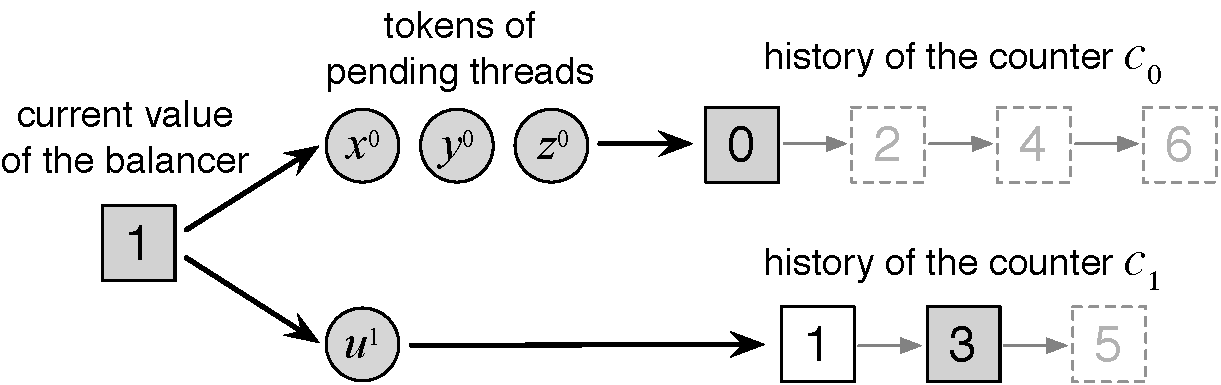
\includegraphics[width=8.2cm]{chist.pdf}      
\caption{Tokens and histories of the simple network}
\label{fig:chist}
\end{figure}
}




% We next list the invariants that describe the interdependence between
% the various components of the real and auxiliary state. 

In addition to $\tkn$ and $\hist$ which come in flavors private to
\emph{self} and \emph{other} threads, we require the following shared
variables: (1) $\heapj$ for the joint heap of the network, and (2)
$b_\joint$, $n^0_\joint$ and $n^1_\joint$ for the contents of $\bal$,
$c_o$ and $c_1$, respectively.

\paragraph{Invariants of the counting network}
\label{sec:count-netw-invar}

The main invariant of the network relates the number of tokens, the
size of histories and the value of the balancer:

\[
\tag{\normalsize{\arabic{tags}}}\refstepcounter{tags}\label{cn:si} 
%
|\hist^0| + |\tkn^0| =
|\hist^1| + |\tkn^1| + b_\joint
\]

The equation formalizes the intuition that out-of-order anomalies of
the counting network appear if one of the two counters is too far
ahead of the other one.
%
The invariant~(\ref{cn:si}) provides a bound on such a situation. One
counter can get ahead temporarily, but then there must be a number of
threads waiting to spend their tokens on the other counter. Thus, the
other counter will eventually catch up.

The approaches such as quiescent and quantitative quiescent
consistency describe this situation by referring to the number of
\emph{unmatched} call events in an event
history~\cite{Derrick-al:FM14,Jagadeesan-Riely:ICALP14}. In contrast,
we formalize this property via auxiliary state: the sets of tokens
$\tknh$ recorded in the entry for the number $t$ determine the
environment's capability to add new history entries, and thus ``run
ahead'' or ``catch up'' after $t$ has been returned.
%
% Such auxiliary state will let us directly specify the network's
% behavior in the moments of quiescence (\ie,~when $\tkno$ is empty),
% but also \emph{quantitatively} bound the out-of-orderness as a
% function of $\tkno$.
%
The other invariants of the counting network are as follows:
%\vspace{2pt}
\begin{enumerate}[label=(\roman*)]

% %
% \[
% \tag{\normalsize{\arabic{tags}}}\refstepcounter{tags}\label{eq:cn-states} 
% {\small
% \begin{array}{r@{\ }c@{\ }l} 
% {\!\!\!\!\!\!\!\!}W_{\ccon} & \!\eqdef & \exists \tkns~\tkno~ \hists~\histo~b~n_0~n_1\ldot 
% %  
% \qcl \spts (\tkns, \hists)\aand \qcl \opts (\tkno, \histo) 
%   \\[4pt] 
% &\aand & \qcl \jpts \bal \hpts b \hunion c_0 \hpts n_0 \hunion c_1 \hpts n_1   
%  \aand \hvalid~(\hists \hunion \histo)         \\[3pt] 
% &\aand & \SI~\tkn^0~\tkn^1~\hist^0~\hist^1~b ~~~~\aand
%          \CI~\hist^0~\hist^1~n_0~n_1 \\[3pt]  
% &\aand & \TI~\tkn^0~\tkn^1~(\hist^0 \hunion \hist^1)\aand \AI~\hist^0~\hist^1~\tkn^0~\tkn^1~n_0~n_1.
% \end{array}
% }
% \]
%

% where $\hist^i = (\hists \hunion \histo)^i$ and
% $\tkn^i = (\tkns \hunion \tkno)^i$ for $i \in \set{0,1}$.

\item\label{cn:state} $\heapj = \bal \mapsto b_\joint \hunion c_0 \mapsto n^0_\joint
  \hunion c_1 \mapsto n^1_\joint$.

\item\label{cn:hvalid} The histories contain disjoint time-stamps. % (\ie $\hists \hunion \histo$ is always defined);
 
% The state-space invariant $W_{\ccon}$ fixes the auxiliary self/other
% components to be pairs of tokens and histories $(\tkns, \hists)$ and
% $(\tkno, \histo)$, which are held/contributed by the thread and its
% environment, correspondingly. The invarian $\hvalid~(\hists \hunion
% \histo)$ ensures that at any moment 
% %
% The joint part of the state contains the pointers $\bal$, $c_0$ and
% $c_1$, and the relations between all these components are specified by
% the invariants $\SI$, $\CI$, $\TI$ and $\AI$.

\item\label{cn:ci} 
%
  The history $\hist^0$ (resp. $\hist^1$) contains \emph{all} even
  (resp. odd) values in $[0, n^0_\joint]$ (resp. $[1, n^1_\joint]$).
%
%    In other words, the network does not ``skip'' values. 
%
    This ensures that $n^0_\joint$ and $n^1_\joint$ are the last
    time-stamps in $\hist^0$ and $\hist^1$, respectively.

\item\label{cn:ti}  
%
  $\tkn^0$, $\tkn^1$ and $\Tomb~(\hists \hunion \histo)$ contain
  mutually disjoint tokens, where $\Tomb~(t \mapsto (\tknh, z) \hunion
  \hist') = \{z\} \hunion \Tomb~\hist'$, and $\Tomb~\emptyset =
  \emptyset$. In other words, a spent token never appears among the
  ``alive'' ones (\ie, in $\tkn^0 \hunion \tkn^1$).

%As a consequence, $\Tomb~(\hists \hunion \histo)$ is always defined.

\item\label{cn:ti1}
%
  $t \mapsto (\tknh, z) \subseteq \hists \hunion \histo
  \implies z \in \tknh$. \\[-7pt]

\item\label{cn:ai} 
%
For any $t$, $\tknh$, $z$: \\[-7pt]
% 
{\small
  \begin{itemize}
  \item   $t \hpts (\tknh, z) \subseteq \hist^0 \implies t + 2\ |\tknh
    \cap \tkn^0| < n^1_\joint + 2\ |\tknh \cap \tkn^1| + 2$, and \\[-7pt]
  \item
    $t \hpts (\tknh, z) \subseteq \hist^1 \implies t + 2\ |\tknh \cap 
    \tkn^1| < n^0_\joint + 2\ |\tknh \cap \tkn^0|
    + 2$.
  \end{itemize}
}
%
\end{enumerate}
\vspace{5pt}
 
\noindent
The invariant~\ref{cn:ai} provides quantitative information about the
network history by relating the actual ($n^0_\joint$, $n^1_\joint$)
and the past ($t$) counter values, via the current amount of
interference ($\tkn$) and the snapshot interference ($\tknh$).
%
To explain~\ref{cn:ai}, we resort to the intuition provided by the
following equality, which, however, being \emph{not quite valid},
cannot be used as an invariant, as we shall see. Focusing on the
first clause in~\ref{cn:ai}, if
$t \mapsto (\tknh, z) \subseteq \hist^0$, then,
intuitively:
%
{\small{
\[
t + 2\ |\tknh^0 \setminus \tkn^0 | + 2\ |\tknh \cap \tkn^0| =
n^1_\joint + 2\ |\tknh \cap \tkn^1| + (2 b_\joint - 1)
\]}}
%
\noindent
The equality says the following. When $t$ is snapshot from $c_0$ and
placed into the history $\hist^0$, the set of outstanding even tokens
was $\tknh^0$. By the present time, $c_0$ has been increased
$|\tknh^0 \setminus \tkn^0|$ times, each time by $2$, thus
$n^0_\joint = t + 2\ |\tknh^0 \setminus \tkn^0|$. What is left to add
to $c_0$ to reach the \emph{period of quiescence}, when no threads
interfere with us, is $2\ |\tknh \cap \tkn^0|$. Similar reasoning
applies to $c_1$. It is easy to see at the period of quiescence, $c_0$
and $c_1$ differ by $2 b_\joint - 1$; that is, the counter pointed to
by $\bal$ is behind by $1$. However, the equality is invalid, as
$b_\joint$ can be read off only in the present, whereas the
``intuitive'' reasoning behind the equality requires a value of
$b_\joint$ from a quiescent period \emph{in the future}. Hence, in
order to get a valid property, we bound $2 b_\joint - 1$ by 2. For
simplicity, we even further weaken the bounds by dropping
$|\tknh^0 \setminus \tkn^0|$ to obtain~\ref{cn:ai}; as it will turn
out, even such a simpler bound will suffice for proving
\textbf{R1}--\textbf{R3}.

% in Section~\ref{sec:qc-client}.

%As already aparent from our explanation, the invariant gives us a way
%to formally model when the network is in the period of quiescence, as
%required in \textbf{R2}, which we verify in
%Section~\ref{sec:qc-client}.
%%

% \gad{I did not find the equation above ``intuitive'' at all. I think
%   it might be better to give the first part of the explanation and
%   introduce the equality. Then, say why it doesn't hold and how to fix
%   it to get a valid invariant. I think that would be easier to
%   understand.}
%
% wontfix
%
% \gad{Also, why the quotation marks around equation? Valid or not, it
%   is still an equality.}
%
% won't fix

\paragraph{Allowed changes in the counting network}
\label{sec:count-netw-prot}


The state of the counting network (auxiliary and real) can be changed
in two possible ways by concurrent threads. These changes formalize
the way the atomic operations \code{flip} and \code{fetchAndAdd2} from
Figure~\ref{fig:counter-fig}~(b) work with auxiliary state.
%
\emph{Flipping} alters the bit value $b_\joint$ of $\bal$ to the
complementary one, $1 - b_\joint$.
%
It also generates a token $z$ (of parity $b_\joint$) and stores it
into $\tkns$. The token is fresh, \ie, distinct from all alive and
spent tokens in $\tkns \hunion \tkno \hunion{\Tomb~(\hists
  \hunion \histo)}$.
%
\emph{Incrementation} spends a token $z$ from $\tkns$, and depending
on its $i$, it atomically increases the value $n^i_\joint$ of $c_i$ by
two, while simultaneously removing $z$ from $\tkns$ (thus, the
precondition is that $z \in \tkns$). It also adds the entry
$(n^i_\joint + 2) \hpts (\tkn^0 \hunion \tkn^1, z^i)$ to $\hists$,
thus snapshoting the values of $\tkn^0$ and $\tkn^1$.
%
It is easy to check that both these allowed changes preserve the
state-space invariants~(\ref{cn:si}), \ref{cn:state}--\ref{cn:ai}, and
that their effect on real state (with auxiliary state erased) are
those of \code{flip} and \code{fetchAndAdd2}.

\subsection{Step 2: a Hoare spec for \texttt{getAndInc}}
\label{sec:spec-gaa}

We now provide a Hoare-style spec for \code{getAndInc}, verified in
our proof scripts. We use the logical variable $\ikn$ and its variants
to range over token sets, and $\gist$ to range over histories.

\[
%
\tag{\normalsize \arabic{tags}}\refstepcounter{tags}\label{eq:qc-spec}
{\small
\!\!\!\!\!\!\!\! 
\begin{array}{c}
  \spec{\!\!
  \begin{array}{c}
    \tkns = \emptyset,
    \hists = \gists,
    \gisto \subseteq \histo,\\[2pt]
    \ikno \subseteq \tkno \hunion (\Tomb~\histo \setminus
    \Tomb~\gisto),
    \Ic{\gisto}{\ikno}
  \end{array}
  \!\!}
  \\\\[-6pt]
  \texttt{getAndInc()}
  % 
  \\[3pt]
  \spec{\!\!\!
  \begin{array}{c}
    \exists \iknh~z \ldot \tkns = \emptyset, 
    \hists = \gists \hunion (\res + 2) \hpts (\iknh, z), 
    \\[2pt]
    \gisto \subseteq \histo, \ikno \subseteq \tkno \hunion (\Tomb~\histo \setminus \Tomb~\gisto), 
    \\[2pt]
    \last~(\gists \hunion \gisto) < 
    \res + 2 + 2~|\iknh \cap \ikno|, 
    \\[2pt]
    \happrox~(\gists \hunion \gisto)~\res~\iknh~z,
     \Ic{\gisto}{\ikno}
  \end{array} 
  \!\!\!} %@\ccon
%
\end{array}
}
\]

The precondition starts with an empty token set ($\tkns = \emptyset$),
and hence by framing, any set of tokens. The initial self-history
$\hists$ is set to an arbitrary $\gists$.\footnote{Alternatively, we
  could have also taken $\hists = \emptyset$, but the clients will
  require generalizing to $\hists = \gists$ by the FCSL's frame
  rule~\cite{Sergey-al:ESOP15}. To save space and simplify the
  discussion, we immediately frame \wrt the auxiliary $\hists$. Our
  examples do not require such client-side framing \wrt~$\tkns$.} The
precondition records the \emph{other} components of the initial state
as follows. First, $\gisto$ names (a subset of) $\histo$, to make it
stable under interference, as in Section~\ref{sec:overview}. Next, we
use $\ikno$ to name the (subset of) initially live tokens
$\tkno$. However, as $\tkno$ may shrink due to other threads spending
tokens, simply writing $\ikno \subseteq \tkno$ is unstable. Instead,
we write $\ikno \subseteq \tkno \hunion (\Tomb~\histo \setminus
\Tomb~\gisto)$ to account for the tokens spent by other threads as
well. The set $\tkno \hunion (\Tomb~\histo \setminus \Tomb~\gisto)$
only grows under interference, as new live tokens are generated, or
old live tokens are spent, making the inclusion of $\ikno$ stable.
%
Indeed, one cannot take \emph{any} arbitrary $\gisto$ and $\ikno$ to
name the \emph{other} components of the initial state. Therefore, we
constrain these two variables by the invariant $\ic$, that relates
them to the \emph{self-}components of the actual state and to each
other according to the
invariants~\ref{cn:hvalid}--\ref{cn:ai}.\footnote{That is, $\gisto$
  and $\ikno$ take the role of $\histo$ and $\tkno$ in
  invariants~\ref{cn:hvalid}--\ref{cn:ai}, with
  $n^i_\joint = \last~(\hists \hunion \gisto)^i$. The formal
  definition of $\ic$ is in our proof scripts.} This is natural,
since, as we will see in Section~\ref{sec:qclients}, all clients
instantiate $\gisto$ and $\ikno$ with the \emph{other}-components of
the actual pre-state, respecting~\ref{cn:hvalid}--\ref{cn:ai}.

% \gad{$ \ikno \subseteq \tkno \hunion (\Tomb~\histo \setminus
%   \Tomb~\gisto)$ breaks awkwardly across lines.}
% wontfix
%
% \gad{I don't get the parentheses around ``a subset of''. It makes it
%   harder to read the phrases, and after all the full subset is still a
%   subset.}
%
% fixed
%
% \gad{I did not get what $\Ic{\gisto}{\ikno}$ is, even after browsing
%   the spec in the code. Is it too long to define it inline? Does it
%   matter altogether?}
%
%   Yes, it does matter. And, yes, it's too long to define it in
%   prose, as it's boring and comes from the fact that SL-ish notation
%   is not a good fit for binary state-constrining postconditions.
%

The postcondition asserts that the final token set $\tkns$ is also
empty (\ie, the token that \code{getAndInc} generates by \code{flip},
is spent by the end). The history $\hists$ is increased by an entry
$(\res + 2) \hpts (\iknh, z)$, corresponding to writing the value of
the result (plus two) into one of the network's counters, snapshoting
the tokens of that moment into $\iknh$, and spending the token $z$ on
the write. $\gisto$ is a subset of the new value of $\histo$, and
$\ikno$ is a subset of the new value of $\tkno \hunion (\Tomb~\histo
\setminus \Tomb~\gisto)$, by the already discussed stability.

The next inequality describes where the entry for $\res + 2$ is placed
\wrt~the pre-state history $\gist = \gists \hunion \gisto$. $\gist$
may have gaps arising due to out-of-order behavior of the network, and
$\res + 2$ may fill one such gap. However, there is a bound on how far
$\res$ (and hence $\res+2$) may be from the tail of $\gist$. We
express it as a function of $\ikno$ and $\iknh$, derived from the
bounds in~\ref{cn:ai}, taking $\res + 2$ for $t$ and
over-approximating the instant value $n_{\joint}^i$ of the
incremented counter via $\last~(\gists \hunion \gisto)$. The
inequality weakens the invariant~\ref{cn:ai}, making it hold for even
and odd entries by moving $2~|\iknh \cap \ikno^i|$ (for $i = 0,1$) to
the right side of $<$ and joining them, since $\ikno^0 \cap \ikno^1 =
\emptyset$.

% To explain it, let us assume that $\res$ is written into $c_1$ and the
% last entry of $\hist$ (let us call it $t$) was written into
% $c_0$. Then, we have a similar ``equation'' as in the explanation
% in~\ref{cn:ai}:
% \[
% t + 2\ |\ikno^0 \setminus \iknh^0| + 2\ |\iknh^0 \cap \ikno^0| = \res
% + |\iknh^1 \cap \ikno^1| + (2 b_\joint -1)
% \]
% To advance $c_0$ to the moment when $\iknh^0$ and $\iknh^1$ were
% recorded, we need to increase $t$ by $2\ |\ikno^0 \setminus
% \iknh^0|$. After that, to advance both $c_0$ and $c_1$ to a quiescent
% period, we have to spend the tokens in $|\iknh^0 \cap \ikno^0|$ (for
% $c_0$) and $|\iknh^1 \cap \ikno^1|$ (for $c_1$). In the quiescent
% period, $c_0$ and $c_1$ differ by $2 b_\joint - 1$. Moving $|\iknh^0
% \cap \ikno^0|$ to the other side of the equation (while not changing
% the sign), omitting $|\ikno^0 \setminus \iknh^0|$, and bounding the
% value of $2 b_\joint - 1$ from above by $2$, we get:
% \[
% t < \res + 2\ |\iknh^0 \cap \ikno^0| + 2 \ |\iknh^1 \cap \ikno^1| + 2
% \]
% which we use in~(\ref{eq:qc-spec}). Being symmetric in $\ikn^0$ and
% $\ikn^1$, the inequality has the pleasant property that it also holds
% in the other three cases: when $\res$ is written into $c_0$ and $t$
% into $c_1$, and when both $\res$ and $t$ are written into the same
% counter, $c_0$ or $c_1$.

% The predicate $\strapprox$, stated next, summarizes several properties
% of the result and the newly introduced history entry, which will be
% crucial for reasoning about clients in Section~\ref{sec:qclients}:
% %
% \[
% \tag{\normalsize \arabic{tags}}\refstepcounter{tags}\label{eq:strapprox}
% %
% \!\!\!\!
% {\small{
% \begin{array}{l}
% \strapprox~\gists~\gisto~\ikno~m_0~m_1~\res~\iknh^0~\iknh^1~z
% ~\eqdef
% \\[2pt]
% ~~~~~~~~~~~~~~~~~~ \sapprox~\ikno~m_0~m_1~\res~\iknh^0~\iknh^1, \\[2pt]
% ~~~~~~~~~~~~~~~~~~ \happrox~(\gists \hunion \gisto)~\res~\iknh^0~\iknh^1~z,\\[2pt]
% ~~~~~~~~~~~~~~~~~~ \tapprox~(\gists \hunion \gisto)~\iknh^0~\iknh^1~z
% \end{array}
% }}
% \]
% %
% \[
% %
% \tag{\normalsize \arabic{tags}}\refstepcounter{tags}\label{eq:sapprox}
% %
% {\small{
% \begin{array}{l}
% \sapprox~\ikn~m_0~m_1~\res~\iknh^0~\iknh^1 ~\eqdef \\[2pt]
% %
% ~~~~  m_0 < \res + 2 + 2 \times (|\iknh^0 \cap \ikn^0| + |\iknh^1 \cap
%   \ikn^1|), \\[2pt]
% ~~~~ m_1 < \res + 2 + 2 \times (|\iknh^0 \cap \ikn^0| + |\iknh^1 \cap
%   \ikn^1|)
% \end{array}
% \hfill
% }}
% \]
% 

%\noindent
Finally, the predicate $\happrox$ provides more bounds that we will
need in the proofs of the client code's properties.
%
\[ 
%
\tag{\normalsize \arabic{tags}}\refstepcounter{tags}\label{eq:happrox}
%
\!\!\!\!\!
{\small{
\begin{array}{l}
\!\!\!\!
\happrox~\gist~\res~\iknh~z \eqdef \hbox{}
\iknh \subseteq \tkno \hunion (\Tomb~\histo) \hunion
  \set{z},\\[2pt]
~~ \forall t~\ikn \ldot t \hpts (\ikn, -) \subseteq \gist \Rightarrow
  z \notin \ikn,~  t < \res + 2 + 2 \ (|\iknh \cap \ikn|)
\end{array}
}}
\]
%
When instantiated with $\gist = \gists \hunion \gisto$, $\happrox$
says the following. The token set $\iknh$ snapshot when $\res+2$ was
committed to history, is a subset of all the tokens in post-state,
including the live ones ($\tkno$), and spent ones ($\Tomb~\histo
\hunion \{z\}$).
%
Moreover, if $t$ is an entry in $\gist$, with contents $(\ikn, -)$,
then: (1) $z \notin \ikn$, because $z$ is a token generated when
\code{getAndInc} executed \code{flip}. Hence, $z$ is fresh \wrt~any
token-set from the pre-state history $\gist$; and (2) $t$ and $\ikn$
satisfy the same bounds \wrt~$\res+2$, as those described for the last
history entry and~$\ikno$.


%\noindent

%
% \begin{comment}
% \paragraph{Why the spec~\eqref{eq:qc-spec} is stable?}
% \label{sec:why-spec-eqrefeq:qc}

% The stability of the spec we ascribed to \code{getAndInc} follows from
% the following observations. First, all clauses in the pre- and
% postconditions that contsrain only \emph{self}-components of the state
% (\eg, $s.\hists = \gists$ or $\tkns = \emptyset$) are stable, since
% they cannot be affected by interference (which might change only
% \emph{other} and \emph{joint} components), as ensured by FCSL's
% meta-theory.
% %
% Second, the stability of all other clauses that also mention the
% \emph{other} component, follows from their \emph{monotonicity} with
% respect to interference. In particular, the union
% $\tkno \hunion \Tomb~\histo$, appearing also in the definition of
% $\happrox$, can only grow, while the union
% $\ikno \hunion \Tomb~\gisto$ is fixed.
% %
% Finally, the rest of the clauses mentions only values that are not
% components of the state being constrained (\eg, $\ikno$, $\gisto$,
% \etc) and, hence, are also unaffected by interference.
% %
% All these stability arguments are carried out as formal proofs in our
% Coq development, accompanying the paper.
% \end{comment}

\paragraph{How will the spec~\eqref{eq:qc-spec} be used?}

The clause $\hists\,{=}\,\gists \hunion (\res+2)\,{\mapsto}\,-$ of
\eqref{eq:qc-spec}, in conjunction with the invariant~\ref{cn:hvalid},
ensures that any two calls to \code{getAndInc}, sequential or
concurrent, yield different history entries, and hence different
results. This establishes~\textbf{R1}, which we will not discuss
further.

The inequality on $\last~(\gists \hunion \gisto)$ will provide
for~\textbf{R2} in client reasoning. To see how, consider the
particular case when $\ikno$ is empty, \ie, the pre-state is
quiescent. In that case, the intersection with $\iknh$ is empty, and
we can infer that $\res + 2$, is larger than either counter's value in
the pre-state. As we shall see in Section~\ref{sec:qclients}, this
captures the essence of QC.

Finally, the predicate $\happrox$~\eqref{eq:happrox} establishes a
bound for the ``out-of-order'' discrepancy between the result $\res$
and any value $t$ committed to the history \emph{in the past}, via
$2~|\iknh \cap \ikn|$. We will further bound this value using the size
of $\iknh$, and the inclusion $\iknh \subseteq \tkno \hunion
\Tomb~\histo$ from~\eqref{eq:happrox}. These bounds will ultimately
enable us to derive the requirement~\textbf{R3}.

% \gad{ The $\hists \ldots$ clause line-breaks bad.}

% \subsubsection{Specifications of {\code{flip}} and
%   {\code{fetchAndAdd2}}}
% \label{sec:qacts}

% The formal verification of the spec~\eqref{eq:qc-spec} follows by
% sequential composition of its operations, \code{flip} and
% \code{fetchAndAdd2}, to which we ascribe the following specs.
% %
% Both specs are obtained by relaxing the definitions of the transitions
% from Section~\ref{sec:count-netw-prot}, \wrt~stability.
% %
% %
% \[
% %
% %\tag{\normalsize \arabic{tags}}\refstepcounter{tags}\label{eq:flip-spec}
% {\small
% %\!\!\!\!\!\!\!\! 
% \begin{array}{c}
%   \spec{\!\!
%   \begin{array}{c}
%     \tkns = \emptyset,
%     \hists = \gists,
%     \gisto \subseteq \histo,\\[2pt]
%     \ikno  \subseteq \tkno \hunion (\Tomb~\histo \setminus
%     \Tomb~\gisto), 
%      \Ic{\gisto}{\ikno}
%   \end{array}
%   \!\!}
%   \\\\[-6pt]
%   \texttt{flip(}\bal\texttt{)}
%   %  
%   \\[3pt]
%   \spec{\!\!
%   \begin{array}{c}
%     \exists b~z^b \ldot \res = (b, z^b)\aand
%     \tkns = \set{z^b}\aand \hists = \gists \aand
%      \Ic{\gisto}{\ikno},
%    \\[2pt]
%     \gisto \subseteq \histo, \ikno \subseteq \tkno \hunion (\Tomb~\histo \setminus \Tomb~\gisto),\\[2pt]    
%     \forall t~\ikn^0~\ikn^1 \ldot
%     t \hpts (\ikn^0, \ikn^1, -) \subseteq (\gists \hunion \gisto) \Rightarrow z^b \notin \ikn^0 \hunion \ikn^1,
%     \\[2pt]     
%     \bapprox~(\last~(\gists \hunion \gisto)^0)~(\last~(\gists \hunion \gisto)^1)~\ikno 
%   \end{array}
%   \!\!}@\ccon
% %
% \end{array}
% }
% \]

% \noindent
% The precondition of \code{flip}'s matches the one of
% \code{getAndInc}. The postcondition contains a clause with a new
% predicate $\bapprox$, relating the last entries $m_0$ and $m_1$ of
% either parity of the initial history $\gist = \gists \hunion \gisto$,
% to the current values $n_\joint^0$ and $n_\joint^1$ of $c_0$ and
% $c_1$.
% %
% \[
% %
% \!\!\!\!
% {\small{
% \begin{array}{l}
% \bapprox~m_0~m_1~\ikno \eqdef \\[2pt]
% %
%   \begin{array}{l}
%    m_0 \le n_\joint^0\aand
%     m_1 + 2 \times |\ikno^1 \cap \tkn^1| < n_\joint^0 + 2 \times
%   |\ikn^0 \cap  \tkn^0| + 2, \\[2pt]
%    m_1 \le n_\joint^1\aand m_0 + 2 \times |\ikno^0 \cap \tkn^0| < n_\joint^1 + 2 \times
%   |\ikn^1 \cap  \tkn^1| + 2 
%   \end{array}
% \end{array}
% \hfill
% }}
% \]
% %
% The predicate says that the contents of $c_0$ and $c_1$ increases,
% hence $m_0$ and $m_1$ are smaller or equal to the current values
% $n_\joint^0$ and $n_\joint^1$, respectively. Moreover, when comparing
% values of different parities (\ie, $m_1$ with $n_\joint^0$ and $m_0$
% with $n_\joint^1$), we require bounds similar to the ones already
% discussed in~\ref{cn:ai} and~\eqref{eq:qc-spec}, and expressed in
% terms of token set $\ikno$ and $\tkn = \tkns \hunion \tkno$, that
% capture the interference in the pre-state and post-state,
% respectively. The predicate is internal to \esc{getAndInc}, and is not
% used by, or even visible to, the clients.

% The precondition of \code{fetchAndAdd2} is the same as \code{flip}'s
% postcondition, and \code{fetchAndAdd2}'s post is the one of
% \code{getAndInc}, so verifying the sequential composition is
% straightforward.
% %
% % We note that the $\bapprox$ property is essential for deriving the
% % inequalities from the postcondition~\eqref{eq:qc-spec}.
% %
% \[
% %
% %\tag{\normalsize \arabic{tags}}\refstepcounter{tags}\label{eq:add-spec}
% {\small
% %\!\!\!\!\!\!\!\!\!\! 
% \begin{array}{c}
%   \spec{\!\!
%   \begin{array}{c}
%    \tkns = \set{z^b}\aand \hists = \gists, 
%      \Ic{\gisto}{\ikno} \aand   \\[2pt]
%     \gisto \subseteq \histo, \ikno  \subseteq \tkno \hunion (\Tomb~\histo \setminus \Tomb~\gisto),\\[2pt]
%     \forall t~\ikn^0~\ikn^1 \ldot
%     t \hpts (\ikn^0, \ikn^1, -) \subseteq (\gists \hunion \gisto) \Rightarrow z^b \notin \ikn^0 \hunion \ikn^1,
%     \\[2pt]    
%     \bapprox~(\last~(\gists \hunion \gisto)^0)~(\last~(\gists \hunion \gisto)^1)~\ikno 
%   \end{array}
%   \!\!}
%   \\\\[-5pt]
%   \texttt{fetchAndAdd2($c_b, \specK{z^b}$)} 
%   % 
%   \\[3pt]
%   {\normalsize{ 
%   \specK{\{}~ {\small\texttt{getAndInc}}\specK{\text{'s post~\eqref{eq:qc-spec},
%   instantiated with}~\gists, \ikno, \gisto\}}@\ccon
%   }}
% %
% \end{array}
% }
% \]

% \noindent
% We note one peculiarity, however. In order to provide a provable spec
% for \code{fetchAndAdd2}, we had to augment its signature with a
% \emph{logical} parameter $\specK{z^b}$, representing the token,
% obtained by executing \code{flip}, to be spent in incrementation of
% $c_b$. While in most Hoare-style specs, logical variables scope over
% the precondition and the postcondition, but do not appear in the code,
% here we had to pass $z^b$ as a function argument.
% %
% This logical parameter serves purely for verification purposes, and
% does not affect the result of the execution. Hence, in principle, it
% can be safely erased, though our current formalization of FCSL in Coq
% does not support such erasure.




\section{Verifying Counting Network's Clients}
\label{sec:qclients}

% We next demonstrate how the spec~\eqref{eq:qc-spec} can be used in
% clients, to establish properties \textbf{R2} and \textbf{R3}. These
% properties have been addressed in the previous work using dedicated
% consistency criteria of quiescent
% consistency~\cite{Aspnes-al:JACM94,Derrick-al:FM14} and quantitative
% quiescent consistency and
% quasi-linearizability~\cite{Afek-al:OPODIS10,Jagadeesan-Riely:ICALP14},
% but here we derive them compositionally, \ie, out of the spec of
% \code{getAndInc}. This will demonstrate the usefulness of Hoare logic
% in deriving properties related to the various flavors of quiescent
% consistency.

Following \textbf{\emph{Step 3}} of our verification method, we now
illustrate requirements \textbf{R2} and \textbf{R3} from the previous
section via two different clients which execute two sequential calls
to \code{getAndInc}. Both clients are higher-order, \ie, they are
parametrized by subprograms, which can be ``plugged in''.
%
The first client will exhibit a quiescence between the two calls, and
we will prove that the call results appear in order, as required by
\textbf{R2}. The second client will experience interference of a
program with a $N$ concurrent calls to \code{getAndInc}, and we will
derive a bound on the results in terms of $N$, as required by
\textbf{R3}.

Both our examples will rely on the general mechanism of hiding,
presented in Section~\ref{sec:background}, as a way to logically restrict the
interference on a concurrent object, in this case, a counting network,
in a lexically-scoped way.
%
To ``initialize'' the counting network data structure, we provide the
starting values for the shared heap ($h_0$) and for the history
($\gist_0$), assuming that the initial set of tokens is empty:
%
% Specifically, we will use the following derived rule:
% %
% {\small{
% \[
% \begin{array}{c}
% \spec{P}~e~\spec{Q} @ \ccon\\[2pt]
% \hline\\[-7pt]
% \!\!\!
% \specK{\{\heaps = \Phi_1(\heapj), \Phi_1(P)\}} \hide_{\Phi_1}~e \specK{\{\exists \Phi_2\ldot \heaps = \Phi_2(\heapj), \Phi_2(Q)\}} @ \cal P
% \end{array}
% \]
% }}
%
\[
\tag{\normalsize \arabic{tags}}\refstepcounter{tags}\label{eq:hide2}
{\small{
\begin{array}{r@{\ }c@{\ }l}
% \text{\normalsize{where}} &
% \Phi_1 & \eqdef & [\emptyset/\tkns, \gist_0/\hists, \heap_0/\heapj,
% \emptyset/\tkno, \histo/\hists] 
% \\[2pt]
\heap_0 & \eqdef & \bal \hpts 0 \hunion c_0 \hpts 0 \hunion c_1 \hpts 1     
\\[2pt]
\gist_0 & \eqdef & \set{0 \hpts (\set{0}, 0), 1 \hpts (\set{1}, 1)}
\end{array}
}}
\]
%
That is, $\gist_0$ provides the ``default'' history for the initial
values 0 and 1 of $c_0$ and $c_1$, with the corresponding tokens
represented by numbers 0 and 1.  As always with hiding, the
postcondition of the hidden program will imply that $\tkno$ and
$\histo$ are both empty, as there is no interference at the end.

% \gad{I think that here, again, the quotation marks around ``plugged in'',
%   ``initialize'', and ``default'' are unnecessary.}

\subsection{Exercising quiescent consistency}
\label{sec:qc-client}

\begin{figure}
\centering
\[
{\small{
\!\!\!\!\!\!\!\!
\begin{array}{c}
  \spec{\!\!
  \begin{array}{c}
    \tkns = \emptyset,
    \hists = \gists,
    \gisto \subseteq \histo, \Ic{\gisto}{\ikno}, \\[2pt]
    \ikno \subseteq \tkno \hunion (\Tomb~\histo \setminus \Tomb~\gisto)
  \end{array}
  \!\!}
\\\\[-5pt]
  \begin{tabular}{c || c}
   $\esc{getAndInc()}$ & ${\small{e_i}}$ 
\end{tabular}
\\\\[-5pt]
~~~~\spec{\!\!
\begin{array}{c}
  \exists \iknh~\gist_i \ldot  
  \tkns = \emptyset\aand \hists = \gbm{\gists \hunion \gist_i \hunion (\res.1 + 2) \hpts (\iknh, -)},\\[1pt]
  \gisto \subseteq \histo\aand \ikno \subseteq \tkno \hunion
  (\Tomb~\histo \setminus \Tomb~\gisto), \Ic{\gisto}{\ikno},\\[1pt]
  \last~(\gists \hunion \gisto)  < \gbm{\res.1} + 2 +
  2~|\iknh \cap \ikno|
%
\end{array}
\!\!} %@\ccon
%
\end{array}
}}  
\]
%
\caption{Parallel composition of \code{getAndInc} and~$e_i$ in~\eqref{eq:eqc}.}
  \label{fig:example1} 
\end{figure}
%



Our first client is the following program~$\eqc$:
%
\[
\tag{\normalsize \arabic{tags}}\refstepcounter{tags}\label{eq:eqc}
{\small{
\begin{array}{ll} 
\Num{1} & (\res_1, -) \Asgn (\esc{getAndInc()} ~||~ e_1) \esc{;} \\[1pt]
\Num{2} & (\res_2, -) \Asgn (\esc{getAndInc()} ~||~ e_2) \esc{;} \\[1pt]
\Num{3} &  \kw{return}~(\res_1, \res_2) 
\end{array}
}}
\]
%
Each of the calls to \esc{getAndInc} interferes with either $e_1$ or
$e_2$, but in the absence of \emph{external} interference, the
quiescent state is reached between the lines 1 and 2. Hence, after
executing $\hide~\eqc$, it should be $\res_1 < \res_2$, following
\textbf{R2}.

The programs $e_1$ and $e_2$ can invoke \code{getAndInc} and modify
the counters concurrently with the two calls of $\eqc$, which we
capture by giving both the following generic spec:
%
\[
%
\tag{\normalsize \arabic{tags}}\refstepcounter{tags}\label{eq:eispec}
{\small
\!\!\!\!\!\!\!\! 
\begin{array}{c}
  \spec{~
  \hists = \emptyset\aand
  \tkns = \emptyset\aand
   \ikn \subseteq \tkno \hunion \Tomb~\histo
  ~}
  \\[1pt]
  e_i
  % 
  \\[1pt]
  \spec{\!\!\!
  \begin{array}{c}
    \exists \gist_i \ldot \hists = \gist_i\aand 
    \tkns = \emptyset\aand 
    \ikn \subseteq \tkno \hunion \Tomb~\histo
  \end{array} 
  \!\!\!} %@\ccon
%
\end{array}
}
\]
%
The postcondition allows for a number of increments via calls to
\esc{getAndInc}, which is reflected in the addition $\gist_i$ to
$\hists$. However, all such calls are required to be \emph{finished}
by the end of $e_i$ ($\tkns = \emptyset$). As customary by now, we use
the logical variable $\ikn$ to name the initial set of \emph{other}
tokens.

Figure~\ref{fig:example1} provides a spec for each of the parallel
compositions in the program~\eqref{eq:eqc}, proved via the
corresponding FCSL inference rule for parallel
composition~\eqref{eq:parrule}.
%
The spec is very similar to~\eqref{eq:qc-spec} with the differences
highlighted via gray boxes: (a) the self-history $\hists$ is increased
by $e_i$'s contribution $\gist_i$ in addition to the entry, introduced
by \code{getAndInc}, (b) the result of the parallel composition is a
pair, but we only constrain its first component $\res.1$, resulting
from the left subprogram. We also drop the last conjunct with
$\happrox$ from~\eqref{eq:qc-spec}, which we won't require for this
example.

%



Next, we use the spec from Figure~\ref{fig:example1} to specify and
verify the program $\eqc$, so far \emph{assuming} external
interference.
%
\[
\!\!\!
{\small{
\begin{array}{c}
\!\!\!\!\!
\spec{\!\!
  \begin{array}{c}
    % \tkns = \emptyset,
    % \gisto \subseteq \histo, \ikno \subseteq \tkno \hunion (\Tomb~\histo \setminus \Tomb~\gisto)\\[2pt]
    % \hists = \gist_0,
    \mbox{Fig.~\ref{fig:example1}'s precondition with $\gists := \gist_0$, $\gisto :=
      \histo$, and $\ikno := \tkno$}
  \end{array}
  \!\!}
  ~\comm{P}
  \\\\[-6pt]
  (\res_1, -) \Asgn (\esc{getAndInc()} ~||~ e_1) \esc{;}
  \\[3pt]
\!\!\!\!{{
\spec{\!\!\!\!
\begin{array}{c}
 \exists \gist_1\ldot \tkns = \emptyset\aand \hists = \gists',~\ldots
% \ikno \subseteq \tkno \hunion (\Tomb~\histo \setminus \Tomb~\gisto),
\\[2pt]
\mbox{where 
 $\gbm{\gists' = \gist_0 \hunion
\gist_1 \hunion (\res_1 + 2)\mapsto -}$, $\gisto := \histo$ and $\ikno :=
\tkno$} 
% \\[2pt]
% \mbox{hence $\Ic{\gisto}{\ikno}$}
  \end{array}
\!\!\!\!}
}}
%
\\\\[-5pt]
(\res_2, -) \Asgn (\esc{getAndInc()} ~||~ e_2) \esc{;}      
\\[3pt]
\spec{\!\!\!\!
\begin{array}{c}
\exists \gist_1~\gist_2~\iknh \ldot     
%
\tkns = \emptyset \aand 
%%\hists = \gists' \hunion \gist_2 \hunion (\res_2 + 2)\mapsto (\iknh, -)\aand\hbox{}\\[2pt] 
\gbm{\ikno \subseteq \tkno \hunion (\Tomb~\histo \setminus \Tomb~\gisto)},\\[1pt]
\gbm{\last~(\gists' \hunion \gisto) < \res_2 + 2 + 2~|\iknh \cap \ikno|},~\ldots 
\end{array}
\!\!\!\!\!}~\comm{Q}
\\\\[-7pt]
~~~~~~~~~~~\kw{return}~(\res_1, \res_2); ~\comm{=: \res} 
\\[2pt]
\spec{~Q(\res.1/\res_1, \res.2/\res_2)~} %@\ccon
\end{array}
}} 
\]
%
We start by instantiating the logical variables $\gists$, $\gisto$ and
$\ikno$ from Figure~\ref{fig:example1} with $\gist_0$, \emph{current}
$\histo$ and $\tkno$, respectively, naming the obtained precondition
$P$.
%
In the following assertion we focus on the clauses constraining
$\tkns$ and $\hists$. To verify the second call, we instantiate
$\gists$, $\gisto$ and $\ikno$ from Figure~\ref{fig:example1} with
$\gists' = \gist_0 \hunion \gist_1 \hunion (\res_1 + 2)\mapsto -$,
\emph{current} $\histo$ and $\tkno$, correspondingly, obtaining the
postcondition, which we name~$Q$.

The inequality in the postcondition $Q$ gives the boundary on the
out-of-order position of $\res_2$ with respect to the \emph{last}
value in the history captured in between the two parallel
compositions. The boundary is given via the size of intersection of
the two sets of tokens: snapshot ($\iknh$) and ``alive'' between the
calls ($\ikno$).
%
Now, to ensure the absence of external interference, we consider the
program $(\hide~\eqc)$.
%
By the general property of hiding (Section~\ref{sec:background}), we
know that at the final state there is no interference, hence $\tkno =
\emptyset$ and $\histo = \emptyset$ in $Q$.
%
Therefore, from the set inclusion on $\ikno$ in $Q$ (the grayed part),
we deduce that $\ikno = \emptyset$.
%
As a consequence, the intersection $\iknh \cap \ikno = \emptyset$, so
from the inequality we obtain
%
\[
%
\tag{\normalsize \arabic{tags}}\refstepcounter{tags}\label{eq:tada1}
%
%{\small{
\begin{array}{c}
 \last~(\gists' \hunion \gisto) < \res.2 + 2
\end{array}
\hfill
%}}
\]
%
%\noindent
%
But $\gists'$ is defined as $(\res.1+2)\mapsto -~\hunion\ldots$,
hence, $\res.1 + 2 \in \mathsf{dom}\ \gists'$, and thus $\res.1 + 2
\le \mathsf{last}\ \gists'$. Even more:
%
\[
%
\tag{\normalsize \arabic{tags}}\refstepcounter{tags}\label{eq:tada2}
%
%{\small{
\begin{array}{c}
\res.1 + 2 \le \last~(\gists' \hunion \gisto).
\end{array}
\hfill
%}}
\]
%
From~\eqref{eq:tada1} and~\eqref{eq:tada2} follows the result
\textbf{R2}: $\res.1 < \res.2$.

\subsection{Proving quantitative bounds}
\label{sec:qqc-client}

We next show how the spec~\eqref{eq:qc-spec} also obtains quantitative
bounds on the out-of-order anomalies in terms of a number of running
threads in the following program $\eqqc$:
%
\[
\tag{\normalsize \arabic{tags}}\refstepcounter{tags}\label{eq:eqqc}
{\small{
\begin{tabular}{l || l}
$
\begin{array}{ll} 
\Num{1} & \res_1 \Asgn \esc{getAndInc();} \\[1pt]
\Num{2} & \res_2 \Asgn \esc{getAndInc();}  \\[1pt]
\Num{3} & \kw{return}~(\res_1, \res_2)
\end{array}
$  
&
$~~~e$
\end{tabular} 
}}
\]
%
The $e$'s spec says that the \emph{number} of calls to \esc{getAndInc}
in~$e$ (\ie, the size of interference $e$ exhibits) is some fixed $N$:
%
\[
%
\tag{\normalsize \arabic{tags}}\refstepcounter{tags}\label{eq:espec}
{\small
\!\!\!\!\!\!\!\!\!  
\begin{array}{c}
  \spec{
  \tkns = \emptyset,
  \hists = \gists }
~  e
~  \spec{\!\!\!
  \begin{array}{c}
    \exists \gist \ldot 
    \tkns = \emptyset,
    \hists = \gists \hunion \gist,
    |\gist| = N
  \end{array} 
  \!\!\!} %@\ccon
%
\end{array}
}
\]
%
Our goal is to prove that in the absence of external interference for
$\eqqc$, $\res_1 < \res_2 + 2 \ N$ (requirement \textbf{R3}).

\begin{figure}
\centering
%    
\[
\!\!\!
{\small{
\begin{array}{c}
  \spec{~
    \mbox{{\normalsize{\eqref{eq:qc-spec}'}}s precondition with $\gists := \gist_0$, $\gisto :=
      \histo$, and $\ikno := \tkno$}~}
% \\\\[-6pt]
% \spec{\!\!
%   \begin{array}{c}
%     \tkns = \emptyset,
%     \hists = \gists,
%     \gisto \subseteq \histo,
%     \ikno \subseteq \tkno \hunion (\Tomb~\histo \setminus \Tomb~\gisto)\\[2pt]
%     \mbox{where $\gisto = \histo$ and $\ikno = \tkno$, hence $\Ic{\gisto}{\ikno}$}
% %    \histo \subseteq \histo,\\[2pt]
% %    \tkno \hunion \Tomb~\histo \subseteq \tkno \hunion \Tomb~\histo
%   \end{array}
%   \!\!}
\\\\[-6pt]
\res_1 \Asgn \esc{getAndInc();}
\\[3pt]
\spec{\!\!
\begin{array}{c}
   \exists \ikn \ldot 
   \tkns = \emptyset, 
   \hists = \gists',
   % \gisto \subseteq \histo, \ikno \subseteq \tkno \hunion
   % (\Tomb~\histo \setminus \Tomb~\gisto)
   \ldots
   \\[2pt]
   \mbox{where $\gbm{\gists' = \gist_0 \hunion (\res_1 + 2) \hpts
       (\ikn, -)}$} 
   % , $\gisto = \histo$ and $\ikno = \tkno$, \ldots}
% \\[2pt]
%    \mbox{hence $\Ic{\gisto}{\ikno}$}
  \end{array}
  \!\!}%
%\\\\[-6pt]
%\spec{\!\!\!
%  \begin{array}{c}
%  \tkns = \emptyset,  
%  \hists = \gists \hunion (\res_1 \!+\! 2) \!\hpts\! (\ikn^0, \ikn^1, -), 
%  \gists' := \hists,\\[2pt] 
%  \gisto := \histo, 
%  \ikno := \tkno,
%  \ikno \hunion \Tomb~\gisto \subseteq \tkno \hunion \Tomb~\histo
%  \end{array}
%  \!\!\!}%
\\\\[-5pt] 
\res_2 \Asgn \esc{getAndInc();}
\\[3pt]
\spec{\!\!\!
\begin{array}{c}
  \exists \iknh~z \ldot     
  % \tkns = \emptyset, \hists = \gists' \hunion (\res_2+2) \mapsto (\iknh, z),\\[2pt]
  \happrox (\gists' \hunion \gisto)~\res_2~\iknh~z, \ldots
\end{array}
\!\!\!}
\\\\[-5pt]
\spec{\!\!\!
\begin{array}{c}
  \exists \iknh~z \ldot     
  % \tkns = \emptyset, \hists = \gists' \hunion (\res_2+2) \mapsto (\iknh^0, \iknh^1, z),\\[2pt]
  \gbm{\iknh \subseteq \tkno \hunion (\Tomb~\histo) \hunion \set{z}},
  z \notin \ikn,\\[2pt] 
  \res_1 + 2 < \res_2 + 2 + 2~|\iknh \cap \ikn|
\end{array}
\!\!\!}
\\\\[-5pt]  
~~~~~~~~~~~~~~~
\kw{return}~(\res_1, \res_2) ~\comm{=: \res}
\\\\[-5pt]
\spec{\!\!\!
\begin{array}{c}
  \res.1 < \res.2 + 2 \ |\tkno \hunion \Tomb~\histo| 
  %
  %\aand\\[1pt] 
  % \tkns = \emptyset\aand
  % \hists = \gists \hunion (\res_1 + 2) \hpts -
  % \hunion (\res_2 + 2) \hpts -
  \end{array}
  \!\!\!} %@\ccon
\end{array}
}} 
\]
%
%
\caption{Proof outline of sequential composition in~\eqref{eq:eqqc}.}
\label{fig:proof2}
\end{figure}

We first verify the sequential composition of the two calls
in~\eqref{eq:eqqc}; the proof outline is in
Figure~\ref{fig:proof2}. 
%
% \ab{Can this proof outline be cut significantly/removed? Can we just
%   give the overall pre-post specs and go directly to the verification
%   of $\eqqc$?}
%
As previously, we start by instantiating the logical variables
$\gists$, $\gisto$ and $\ikno$ from spec~\eqref{eq:qc-spec} with
$\gists$, $\histo$ and $\tkno$, respectively. In the assertion,
resulting by of the first \esc{getAndInc}, we keep only the clauses
involving $\tkns$ and $\hists$, dropping the rest.
%
To verify the second \esc{getAndInc} call, we instantiate $\gists$,
$\gisto$ and $\ikno$ with $\gists' = \gists \hunion (\res_1+2) \mapsto
(\ikn, -)$, current $\histo$ and $\tkno$.

In the postcondition of the second call to \esc{getAndInc}, we focus
on the $\happrox~(\gists' \hunion \gisto)~\res_2~\iknh~z$ clause,
where $\iknh$ is the set of tokens snapshot when contributing
$\res_2+2$.
%
Unfolding the definition of $\happrox$ from~\eqref{eq:happrox}, we
obtain $\iknh \subseteq \tkno \hunion \Tomb~\histo
\hunion\{z\}$. Also, using $(\res_1 +2)\mapsto (\ikn, -)$ in the
implication that the unfolding obtains, we get $z \notin \ikn$ and
\[
\tag{\normalsize \arabic{tags}}\refstepcounter{tags}\label{eq:le0}
{\small{\res_1 + 2 < \res_2 + 2 + 2~|\iknh \cap \ikn|
}}
\]
%
Now we use the following trivial fact to simplify.
%
\vspace{8pt}
%
\begin{lemma}
\label{lm:intersect2}
If $z \in \iknh$ and $z \notin \ikn$, then $|\iknh \cap \ikn| \le
|\iknh| - 1$.
\end{lemma}
%
%
\vspace{8pt}
%
\noindent
Using the invariant~\ref{cn:ti1}, Lemma~\ref{lm:intersect2}
derives
$|\iknh \cap \ikn| \le |\iknh| - 1$
%
after which, the inclusion $\iknh \subseteq \tkno
\hunion \Tomb~\histo \hunion \set{z}$ leads to
%
\[
\tag{\normalsize \arabic{tags}}\refstepcounter{tags}\label{eq:le5}
{\small{
|\iknh \cap \ikn| \le |\tkno \hunion \Tomb~\histo|}}
\]
%
Combined with~\eqref{eq:le0}, this gives us $\res_1 < \res_2 + 2 \
|\tkno \hunion \Tomb~\histo|$, as shown in Figure~\ref{fig:proof2}'s
postcondition. In words, it asserts that the discrepancy between
$\res.1$ and $\res.2$ is bounded by the size of the tokens, which are
either held by the interfering threads at the end or are spent.
%
% \gad{low-priority right now, but still: the inequality above spreads
%   across a linebreak, and worse, in the middle of the arguments for an
%   operator.}
%
% \is{won't fix}

\begin{figure}[t]
  \centering
\[
{\small{
\!\!\!\!\!\!\!\!
\begin{array}{c}
  ~~~~~~~~\spec{~
  \tkns = \emptyset,
  \hists = \gist_0, \ldots
~} ~\comm{P}
\\[2pt]
  \begin{tabular}{c || c}
$
\spec{\!\!\!
    \begin{array}{c}
    \tkns = \emptyset,
    \hists = \gist_0
  \end{array}\!\!\!}
$
&
$
\spec{\!\!\!\begin{array}{c}
    \tkns = \emptyset,
    \hists = \emptyset
  \end{array}\!\!\!}
$
\\[3pt]
   $\begin{array}{l}
      \res_1 \Asgn \esc{getAndInc();}\\[1pt]
      \res_2 \Asgn \esc{getAndInc();}\\[1pt]
      \kw{return}~(\res_1, \res_2) ~\comm{ =: \res}\!\!\!
    \end{array}$
\!\!\!\!\!\!
& ${\small{e}}$ 
\\\\[-5pt] 
$
\spec{\!\!\!
{\small{
  \begin{array}{c}
    \res.1 < \res.2 + 2 \ |\tkno \hunion \Tomb~\histo|
  \end{array}
}}
  \!\!\!}\!\!$
\!\!
&
\!\!$\spec{\!\!\!
{{
  \begin{array}{c}
    \exists \gist \ldot 
    \hists = \gist, 
    |\gist| = N,
    \ldots
  \end{array}
}}
\!\!\!}$
\end{tabular}
\\\\[-5pt]
\comm{\res_1 := \res.1.1, \res_2 := \res.1.2}
\\\\[-6pt]
\spec{
\res_1 < \res_2 + 2 \ |\tkno \hunion \Tomb~(\histo \hunion \gist)|
}
\\[3pt]
~~~~~~~~\spec{
\res_1 < \res_2 + 2 \ |\tkno \hunion \Tomb~\histo| + 2 \ N
} ~\comm{Q}
%
\end{array}
}}  
\]
  \caption{Proof outline for the $\eqqc$ program.}
  \label{fig:eqqcproof}
\end{figure}

Figure~\ref{fig:eqqcproof} shows the proof outline for $\eqqc$ via the
spec from Figure~\ref{fig:proof2}.
%
By the parallel composition rule~\eqref{eq:parrule}, the precondition
splits into two subjective views, where we send the initial history
$\gist_0$ to the left thread, and the empty history to the right
thread. The proof from Figure~\ref{fig:proof2} then applies to the
left thread, and the spec~\eqref{eq:espec} applies to the right
one. Final $\histo$ of the left thread is the union of $\histo$ from
the joined thread with $\gist$, since the environment of the left
thread includes the right thread and of the join. Rewriting by this
property in the postcondition of the left thread gives us the post of
the joint thread: $\res_1 < \res_2 +2\ |\tkno \hunion \Tomb~(\histo
\hunion \gist)|$, which we can next simplify into
\[
\res_1 < \res_2 + 2\ |\tkno \hunion \Tomb~\histo| + 2\ N
\]
because $\Tomb$ distributes over $\hunion$, and $|\Tomb~\gist| =
|\gist| = N$. Finally, we restrict the external interference by
considering $(\hide~\eqqc)$. From the properties of hiding,
we deduce that $\tkno$ and $\histo$ in $Q$ are empty, hence we can
simplify into $\res_1 < \res_2 + 2 \ N$, which is the desired
result~\textbf{R3}.
%
%\gad{The same happens here, just before the highlighted math.}

\section{Discussion, Limitations and Future Work}
\label{sec:limitations}



\section{Related Work}
\label{sec:related}

% Existing methods for specifying the behavior of concurrent data
% structures and programs are either history-based or state-based.
% %
% The former ones describe the behavior of an object by describing and
% characterizing call/return strings that can be obtained by invoking
% the methods concurrently by several threads. 
% %
% The later ones define the object's behavior by posing requirements to
% a state, in which object's methods are safe to run, and stating
% assertions over a state, resulting from the object's method call. The
% second group of approaches employs program logics as a way to specify
% the state of interest as well as a mechanism to compose the program
% specifications.

% This paper contributes to the goal of unifying the history- and
% state-based views to specification and verification of concurrent
% objects.

% In this section we describe related approaches for reasoning about
% concurrency that have motivated our work.

\paragraph{Linearizability and history-based criteria.}

% In the past 25 years, linearizability has been widely applied to
% capture the behavior of concurrent objects with intuitive sequential
% specifications, and even suitable for automatic synthesis of some
% concurrent objects~\cite{Vechev-Yahav:PLDI08}. Thanks to the
% compositional proof method, based on \emph{linearization points},
% proofs of linearizability in most of the cases are amenable for
% practical computer-aided
% verification~\cite{Burckhardt-al:PLDI10,Derrick-al:TOPLAS11,Vafeiadis:CAV10,Amit-al:CAV07,Shacham-al:OOPSLA11,Dragoi-al:CAV13}.

The need for correctness criteria alternative to
linearizability~\cite{Herlihy-Wing:TOPLAS90}, which is more relaxed
yet compositional, was recognized in the work on counting
networks~\cite{Aspnes-al:JACM94}.
%
The suggested notion of quiescent
consistency~\cite{Shavit-Zemah:TOPLAS96} required the operations
separated by a quiescent state to take effect in their logical order.
%
%
A more refined correctness condition, \emph{quasi-linearizability},
implementing a relaxed version of linearizability with an upper bound
on nondeterminism, was proposed by Afek~\etal~\cite{Afek-al:OPODIS10},
allowing them to obtain the quantitative boundaries similar to what we
proved in Section~\ref{sec:qqc-client}.
%
The idea of relaxed linearizability was later used in the work on
\emph{quantitative relaxation} (QR)~\cite{Henzinger-al:POPL13} for
designing scalable concurrent data structures by changing the
specification set of sequential histories.
%
Most recently, \emph{quantitative quiescent consistency} has been
proposed as another criterion incorporating the possibility to reason
about effects of bounded thread
interference~\cite{Jagadeesan-Riely:ICALP14}.
%
It is worth noticing that some of these correctness criteria are
incomparable (\eg, QC and QR~\cite{Henzinger-al:POPL13}, QL and
QQC~\cite{Jagadeesan-Riely:ICALP14}) hence, for a particular
concurrent object, choosing one or another criterion should be
justified by the needs of the object's client. Therefore, a suitable
correctness condition is essentially ``\emph{in the eye of the
  beholder}'', as is typical in programming, when designing libraries
and abstract data structures, and the logic-based approach we advocate
provides precisely this flexibility in choosing desired specs.

% However, how suitable is one or another relaxed correctness
% condition %from the listed ones
% for reasoning about safety properties of a particular client program
% is still largely an open question.

\paragraph{Hoare-style specifications of concurrent objects.}
\label{sec:related-logic-based}

% Program logics for concurrency allow one to capture in the
% specification precisely those bits of information about the program's
% state, which are relevant for the program's clients, making it
% possible to abstract over the irrelevant details of the
% implementation~\cite{DinsdaleYoung-al:ECOOP10}.

Hoare-style program logics were used with great success to verify a
number of concurrent data structures and algorithms, which are much
more natural to specify in terms of observable state modifications,
rather than via call/return histories. The examples of such objects
and programs include
barriers~\cite{Dodds-al:POPL11,Hobor-Gherghina:ESOP11}, concurrent
indices~\cite{ArrozPincho-al:OOPSLA11}, flat
combiner~\cite{Turon-al:ICFP13,Sergey-al:ESOP15}, event
handlers~\cite{Svendsen-Birkedal:ESOP14}, shared graph
manipulations~\cite{Raad-al:ESOP15,Sergey-al:PLDI15}, as well as their
multiple client programs.
%
The observation about a possibility of using program logics as a
correctness criterion, alternative to linearizability, has been made
in some of the prior
works~\cite{Jacobs-Piessens:POPL11,ArrozPincho-al:OOPSLA11,Svendsen-al:ESOP13}.
%
Their criticism of linearizability addressed its inability to capture
the state-based properties, such as dynamic memory
ownership~\cite{Jacobs-Piessens:POPL11}---something that
linearizability indeed cannot tackle, unless it's
extended~\cite{Gotsman-Yang:CONCUR12}.
%
However, we are not aware of any prior attempts to capture CAL, QC and
QQC-like properties of concurrent executions by means of \emph{one and
  the same} program logic and employ them in client-side
reasoning.

%
% Verification in such logics is done structurally, \ie, by
% systematically applying syntax-directed inference rules, until the
% spec is proved. Several mechanized tools for logic-based
% concurrent reasoning have been
% released~\cite{Sergey-al:PLDI15,Appel-al:BOOK14}.

Several logics for proving linearizability or, equivalently,
observational refinement~\cite{Filipovic-al:TCS10,Turon-al:POPL13},
have been proposed
recently~\cite{Turon-al:ICFP13,Liang-Feng:PLDI13,Vafeiadis:PhD}, all
employing variations of the idea of using \emph{specifications as
  resources}, and identifying (possibly, non-fixed or non-local)
linearization points, at which such specification should be ``run''.
%
In these logics, after establishing linearizability of an operation,
one must still devise its Hoare-style spec, such that the spec is useful for
the clients.
% %
% To avoid this detour, a number of other logic-based approaches have
% suggested to assign Hoare-style specifications \emph{directly} to
% fine-grained object
% implementations~\cite{Svendsen-al:ESOP13,Svendsen-Birkedal:ESOP14,ArrozPincho-al:ECOOP14}
% and reason out of these specs.

Similarly to the way linearizability allows one to replace a
concurrent operation by an atomic one, several logics have implemented
the notion of \emph{logical atomicity}, allowing the clients of a data
structure to implement application-specific synchronization on top of
the data structure operations.
%
Logical atomicity can be implemented either by parametrizing specs
with client-specific auxiliary
code~\cite{Jacobs-Piessens:POPL11,Svendsen-al:ESOP13,Svendsen-Birkedal:ESOP14,Jung-al:POPL15}
or by engineering dedicated rules relying on the simulation between
the actual implementation and the ``atomic''
one~\cite{ArrozPincho-al:ECOOP14}.
%
% Both approaches to logical atomicity require one to identify precisely
% a \emph{synchronization point}~\cite{Svendsen-al:ESOP13} within the
% structure being verified, which makes it non-trivial to apply them for
% specifying non-linearizable objects, especially when conducting
% quantitative logic-based reasoning, which we demonstrated in
% Section~\ref{sec:qqc-client}.

Instead of trying to extend the existing approaches for logical
atomicity to non-linearizable objects (for which the notion of
atomicity is not intuitive), we relied on a general mechanism of
auxiliary state, provided by FCSL~\cite{Nanevski-al:ESOP14}. 
%
Specifically, we adopted the idea of histories as auxiliary
state~\cite{Sergey-al:ESOP15}, which, however, was previously explored
in the context of FCSL only for specifying linearizable structures.
%
% Similarly to logical atomicity, the histories-as-state specification
% approach makes fine-grained concurrent programs look like atomic ones,
% since due to compositionality, the specification clients only see the
% history entries.
%
% 
We introduced enhanced notation for referring directly to histories
(\eg, $\hists$, $\histo$), although FCSL's initial logical
infrastructure and inference rules remained unchanged.

% Recently, attempts were made to unify the common idioms occurring in a
% number of concurrency logics in a generic framework of
% \emph{Views}~\cite{DinsdaleYoung-al:POPL13}.
% %
% However, that result is orthogonal to our findings, as \emph{Views}
% are a framework for proving logics sound, not to prove programs, and
% this paper, we focused on using a particular logic (FCSL) for specifying a
% new class of concurrent data structures.
The purpose of \emph{Views}~\cite{DinsdaleYoung-al:POPL13} is to provide a PCM-based semantic framework for proving soundness of logics and type systems, and thus to unify common idioms occurring in several recent concurrency logics. However, the framework has not used PCMs for auxiliary state and/or specification of user programs. \ab{Please check.}


In this work, we do not argue that FCSL is the only logic capable of
encoding custom correctness conditions and their combinations, though,
we are not aware of any other work exploring a similar possibility.
%
However, we believe that FCSL's explicit \emph{other}
subjective state component provides the most straightforward way to do
so.
%
The logics like CAP~\cite{DinsdaleYoung-al:ECOOP10} and
TaDA~\cite{ArrozPincho-al:ECOOP14}, from our experience and personal
communication with their authors, may be capable of implementing our
approach at the expense of engineering a much more complicated
structure of capabilities to encode histories and their invariants,
and ``snapshot'' interference of an environment.
%
Other logics incorporating the generic PCM
structure~\cite{Raad-al:ESOP15,Jung-al:POPL15,Jung-al:ICFP16,Turon-al:OOPSLA14}
might be able to implement our approach, although none of these logics
provide an FCSL-style rule for hiding~\eqref{eq:ehide} as a uniform
mechanism to express explicit quiescence.

%\todo{State that in our cases histories are per-object.}

Concurrently with this work, Hemed~\etal developed a (not yet
mechanized) verification technique for CAL~\cite{Hemed-al:DISC15},
which they applied to the exchanger and the elimination
stack. Similarly to our proposal, they specify CAL-objects via Hoare
logic, but using one global auxiliary history, rather than subjective
auxiliary state. 
%
This tailors their system specifically to CAL (without a possibility
to incorporate reasoning about other, non CA-linearizable, concurrent
structures), and to programs with a \emph{fixed} number of threads. In
contrast, FCSL supports dynamic thread creation, and is capable of
uniformly expressing and mechanically verifying several different
criteria, with CAL merely a special case, obtained by a special choice
of PCM. Moreover, in FCSL the criteria combine, as illustrated in
Section~\ref{sec:cal}, where we combined quiescence with CAL via
hiding. Hiding is crucial for verifying clients with explicit
concurrency, but is currently unsupported by Hemed~\etal's method.
%
% Related is the property of our histories that no event may appear
% between two twin timestamps. We used this property to verify the
% client in Section~\ref{sec:cal}, but this does not seem to hold for
% histories used by Hemed~\etal

%Concurrently with our work, Hemed~\etal developed a (not yet
%mechanized) verification technique for
%CAL~\cite{Hemed-al:DISC15}. Similarly to our proposal, they employed
%the idea of specifying CAL-objects via Hoare triples with auxiliary
%histories. Unlike our approach, their choice of abstractions is
%tailored for conducting proofs about CAL, and they don't establish a
%soundness result of their Hoare-style specs, with respect to CAL or
%any other semantics. In contrast, what we propose is using a uniform
%framework, proved sound from first principles~\cite{Sergey-al:PLDI15},
%capable of capturing the essence of multiple correctness conditions
%(including CAL) and verifying them mechanically. Our spec of the
%exchanger~\eqref{tag:exchangespec} can be easily generalized to tackle
%verification of the elimination stack (main example
%from~\cite{Hemed-al:DISC15}) by parametrizing it with a
%client-provided invariant on histories. Furthermore, by using FCSL as
%a logical foundation, we can also reason about quiescence (via hiding)
%and dynamic thread spawning (via the rule~\eqref{eq:parrule}). These
%components are crucial for verifying clients featuring explicit
%concurrency (Section~\ref{sec:cal}), and we currently don't see how to
%conduct such proofs out of the spec from~\cite{Hemed-al:DISC15}.


% \paragraph{Reasoning about linearizability in program logics}
% \label{sec:rel-linear}

% \begin{itemize}

% \item Logics for linearizability (viktor's PhD), LF, Turon, contextual refinement

% \item Hindsight paper by O'Hearn and company

% \item Observation from the HOCAP paper about the push2 method, that,
%   however, never were extended to any interesting structures, so we
%   did it.

% \item Abstract atomicity

% \end{itemize}


%\vspace{-4pt}

\section{Conclusion and Future Work}
\label{sec:conclusion}

%\vspace{-2pt}

In this paper we have presented a number of formalization techniques,
enabling specification and verification of highly scalable
non-linearizable concurrent objects and their clients in Hoare-style
program logics.
%
Specifically, we have explored several reasoning patterns, all
involving the idea of formulating execution histories as an instance
of auxiliary state and then making these histories to be a subject of
object-specific invariants, capturing the expected concurrent object
behavior.
%
In particular, we have discovered that quantitative logic-based
reasoning about concurrent behaviors can be done by storing relevant
information about interference directly into the entries of a logical
auxiliary history, a pattern which we later demonstrated to be
beneficial in the client-side proofs.

We believe that our results help to bring the Hoare-style reasoning
approach into the area of non-linearizable concurrent data structures
and open a number of exciting opportunities for the field of
logic-based concurrency verification.

For instance, by ascribing interference-sensitive quantitative specs
in the spirit of~\eqref{eq:qc-spec} to relaxed concurrent
libraries~\cite{Henzinger-al:POPL13}, one can assess the applicability
of a particular library implementation for its clients, that can
tolerate the anomalies caused by interference, as long as they can
logically infer the desired safety assertions from the library spec,
as we did in Section~\ref{sec:qclients}.
%
Since logical approaches enable reasoning about higher-order
concurrent data
structures~\cite{Svendsen-al:ESOP13,Turon-al:ICFP13,Sergey-al:ESOP15},
we envision the possibility of giving parametric logical specs to such
generic relaxed constructions as diffracting/elimination
trees~\cite{Shavit-Touitou:TCS97,Shavit:CACM11} that, once
instantiated with suitably specified stacks or pools on the leaves,
would yield a provably correct, highly scalable concurrent container
implementation.


% Acknowledgements:

% Michael Emmi
% Pierre Ganty
% Andrea Cerone
% Anton Podkopaev

% \todo{Generalizing the construction of the counting network to
%   arbitrary diffracting trees}

% \todo{Elimination and diffracting trees~\cite{Shavit-Touitou:TCS97}.}



% \acks
% \todo{Acknowledgments, if needed.}

%\newpage

\setlength{\bibsep}{2.5pt}
\bibliographystyle{abbrv}
\softraggedright 
\bibliography{bibmacros,references,proceedings}


\end{document}


